
\documentclass[12pt, a4paper]{report}

% Suport pentru diacritice și alte simboluri
\usepackage{fontspec}

% Suport pentru mai multe limbi
\usepackage{polyglossia}

% Setează limba textului la română
\setdefaultlanguage{romanian}
% Am nevoie de engleză pentru rezumat
\setotherlanguages{english}

% Indentează și primul paragraf al fiecărei noi secțiuni
\SetLanguageKeys{romanian}{indentfirst=true}

% Suport pentru diferite stiluri de ghilimele
\usepackage{csquotes}

\DeclareQuoteStyle{romanian}
  {\quotedblbase}
  {\textquotedblright}
  {\guillemotleft}
  {\guillemotright}

% Utilizează biblatex pentru referințe bibliografice, cu un singur stil de
% citare numeric (bibliografie numerotată în ordinea citării în text,
% conform ghidului de redactare al facultății)
\usepackage[
    maxbibnames=50,
    sorting=none,
    style=numeric,
    giveninits=true
]{biblatex}

\addbibresource{bibliography.bib}

\AtBeginDocument{%
  % Elimină conjuncția ("și") dintre ultimii doi autori -- doar virgulă
  % între nume, ca în exemplul din ghidul de redactare.
  \DeclareDelimFormat{finalnamedelim}{\multinamedelim}%
  % Nu prefixa adresa web cu "URL:" -- afișeaz-o brut, ca în exemplul din
  % ghid.
  \DeclareFieldFormat{url}{\url{#1}}%
  % Formatul cerut pentru data accesării resurselor online:
  % "[accesat: ZZ.LL.AAAA]", în loc de formatul implicit
  % "(accesat în Z.L.AAAA)".
  \DeclareFieldFormat{urldate}{\mkbibbrackets{accesat: #1}}%
}

% Zerourile de umplutură pentru ziua/luna datei de accesare (ex. "01.09.2026"
% în loc de "1.9.2026") trebuie redefinite ca extra de limbă românească --
% romanian.lbx își reaplică propria definiție a \mkbibdateshort chiar
% înainte de a tipări bibliografia, ceea ce ar anula o redefinire făcută
% mai devreme (ex. în \AtBeginDocument).
\newcommand{\thesiszeropad}[1]{\ifnum#1<10 0\fi#1}
\DefineBibliographyExtras{romanian}{%
  \renewcommand*{\mkbibdateshort}[3]{%
    \iffieldundef{#3}{}{\thesiszeropad{\thefield{#3}}\adddot}%
    \iffieldundef{#2}{}{\thesiszeropad{\thefield{#2}}\adddot}%
    \iffieldbibstring{#1}
      {\bibstring{\thefield{#1}}}
      {\dateeraprintpre{#1}\mkyearzeros{\thefield{#1}}}}%
}

% Setează spațiere inter-linie la 1.5
\usepackage{setspace}
\onehalfspacing

% Modificarea geometriei paginii
\usepackage{geometry}

% Include funcțiile de grafică
\usepackage{graphicx}
% Încarcă imaginile din directorul `images` și din graficele generate pentru
% capitolele de metodologie / rezultate / explicabilitate
\graphicspath{
    {./images/}
    {../../data/graphs/EDA/credit_card/}
    {../../data/graphs/EDA/yahoo/}
    {../../data/graphs/EDA/cicids/}
}

% Tabele și figuri fixate (folosite în capitolele de metodologie/rezultate)
\usepackage{booktabs}
\usepackage{float}

% Rânduri ușor mai compacte în tabele (economisește spațiu vertical fără a
% reduce dimensiunea fontului)
\renewcommand{\arraystretch}{0.85}

% Listări de cod
\usepackage{listings}

% Linkuri interactive în PDF
\usepackage[
    colorlinks,
    linkcolor={black},
    menucolor={black},
    citecolor={black},
    urlcolor={blue}
]{hyperref}

% Permite ruperea URL-urilor lungi din \url{} la orice caracter, evitând
% cutii "overfull" în paragrafele/footnote-urile care le conțin
\usepackage{xurl}

% Simboluri matematice codificate Unicode
\usepackage[warnings-off={mathtools-colon,mathtools-overbracket}]{unicode-math}

% Comenzi matematice
\usepackage{amsmath}
\usepackage{mathtools}

% Formule matematice
\newcommand{\bigO}[1]{\symcal{O}\left(#1\right)}
\DeclarePairedDelimiter\abs{\lvert}{\rvert}

% Suport pentru rezumat în două limbi
% Bazat pe https://tex.stackexchange.com/a/70818
\newenvironment{abstractpage}
  {\cleardoublepage\vspace*{\fill}\thispagestyle{empty}}
  {\vfill\cleardoublepage}
\renewenvironment{abstract}[1]
  {\bigskip\selectlanguage{#1}%
   \begin{center}\bfseries\abstractname\end{center}}
  {\par\bigskip}

% Suport pentru anexe
\usepackage{appendix}

% Stiluri diferite de headere și footere
\usepackage{fancyhdr}

% Permite modificarea comenzii \chapter (eliminarea saltului de pagină)
\usepackage{etoolbox}

% Metadate
\title{Analiza paradigmelor de anomaly detection pe seturi de date cu structură temporală diferită}
\author{Savin Radu-Andrei}

% Generează variabilele cu @
\makeatletter

% Împiedică \chapter să înceapă întotdeauna pe o pagină nouă. Se înlocuiește
% saltul de pagină cu \par (nu se elimină complet), altfel titlul de capitol
% se lipește de sfârșitul paragrafului anterior, pe aceeași linie.
\patchcmd{\chapter}{\if@openright\cleardoublepage\else\clearpage\fi}{\par}{}{%
  \typeout{Nu s-a putut elimina saltul de pagină din \string\chapter.}%
}

% Reduce spațiul vertical din titlul de capitol (implicit gândit pentru
% începutul unei pagini noi -- \vspace*{50pt} înainte, \vskip 40pt după --
% ceea ce lasă un gol mare, nepotrivit, în mijlocul paginii acum că
% \chapter nu mai forțează o pagină nouă). Se patchează valorile de
% spațiere direct în interiorul macro-urilor existente, fără a le
% rescrie complet.
\patchcmd{\@makechapterhead}{\vspace*{50\p@}}{\vspace*{10\p@}}{}{%
  \typeout{Nu s-a putut reduce \string\vspace* de dinaintea titlului de capitol (numerotat).}%
}
\patchcmd{\@makechapterhead}{\vskip 20\p@}{\vskip 6\p@}{}{%
  \typeout{Nu s-a putut reduce \string\vskip dintre numărul și titlul capitolului.}%
}
\patchcmd{\@makechapterhead}{\vskip 40\p@}{\vskip 15\p@}{}{%
  \typeout{Nu s-a putut reduce \string\vskip de după titlul de capitol (numerotat).}%
}
\patchcmd{\@makeschapterhead}{\vspace*{50\p@}}{\vspace*{10\p@}}{}{%
  \typeout{Nu s-a putut reduce \string\vspace* de dinaintea titlului de capitol (nenumerotat).}%
}
\patchcmd{\@makeschapterhead}{\vskip 40\p@}{\vskip 15\p@}{}{%
  \typeout{Nu s-a putut reduce \string\vskip de după titlul de capitol (nenumerotat).}%
}

\begin{document}

% Front matter
\cleardoublepage
\let\ps@plain

% Pagina de titlu
\begin{titlepage}

% Redu marginile
\newgeometry{left=2cm,right=2cm,bottom=1cm}

\begin{figure}[!htb]
    \centering
    \begin{minipage}{0.2\textwidth}
        
\includegraphics[width=\linewidth]{logo-ub.png}
    \end{minipage}
    \begin{minipage}{0.5\textwidth}
        \large
        \vspace{0.2cm}
        \begin{center}
            \textbf{UNIVERSITATEA DIN BUCUREȘTI}
        \end{center}
        \vspace{0.3cm}
        \begin{center}
            \textbf{
                FACULTATEA DE \\
                MATEMATICĂ ȘI INFORMATICĂ
            }
        \end{center}
    \end{minipage}
    \begin{minipage}{0.2\textwidth}
        
\includegraphics[width=\linewidth]{logo-fmi.png}
    \end{minipage}
\end{figure}

\begin{center}
\textbf{SPECIALIZAREA INFORMATICĂ}
\end{center}

\vspace{1cm}

\begin{center}
\Large \textbf{Lucrare de licență}
\end{center}

\begin{center}
\huge \textbf{\MakeUppercase{\@title}}
\end{center}

\vspace{3cm}

\begin{center}
\large \textbf{Absolvent \\ \@author}
\end{center}

\vspace{0.25cm}

\begin{center}
\large \textbf{Coordonator științific \\ Paul Irofti}
\end{center}

\vspace{2cm}

\begin{center}
\Large \textbf{București, septembrie 2026}
\end{center}
\end{titlepage}
\restoregeometry
\newgeometry{
    margin=2.3cm
}

\fancypagestyle{main}{
  \fancyhf{}
  \renewcommand\headrulewidth{0pt}
  \fancyhead[C]{}
  \fancyfoot[C]{\thepage}
}

\addtocounter{page}{1}

% Rezumatul
\begin{abstractpage}

\begin{abstract}{romanian}
Această lucrare investighează în ce măsură modul în care un model de detecție a anomaliilor reprezintă structura latentă a datelor \enquote{normale} determină tipurile de anomalii pe care le poate detecta. Șapte modele, acoperind patru paradigme structural distincte (graniță, partiționare, bottleneck de compresie, obiectiv predictiv), sunt evaluate printr-un pipeline uniform pe trei seturi de date cu grade diferite de structură temporală -- tranzacții bancare tabelare, serii de timp Yahoo Webscope S5 și fluxuri de rețea CIC-IDS2017.
Rezultatele arată că performanța fiecărei paradigme depinde sistematic de tipul de anomalie și de structura datelor, nu de puterea intrinsecă a modelului, iar o serie de studii de caz de explicabilitate confirmă direct mecanismele propuse pentru a explica aceste diferențe.
Un ansamblu construit pe baza a două paradigme cu evidențe demonstrabil disjuncte extinde acoperirea pe clase de atac altfel nedetectabile individual, confirmând valoarea combinării unor asumpții complementare despre normalitate.
\end{abstract}

\begin{abstract}{english}
This thesis investigates the extent to which the way an anomaly detection model represents the latent structure of \enquote{normal} data determines the types of anomalies it can detect. Seven models, spanning four structurally distinct paradigms (boundary, partitioning, compression bottleneck, predictive objective), are evaluated under a uniform pipeline across three datasets with varying degrees of temporal structure -- tabular credit card transactions, Yahoo Webscope S5 time series, and CIC-IDS2017 network flows.
Results show that each paradigm's performance depends systematically on the type of anomaly and the structure of the data, rather than on the model's intrinsic strength, and a series of explainability case studies directly confirm the mechanisms proposed to explain these differences.
An ensemble built from two paradigms with demonstrably disjoint evidence extends coverage to attack classes otherwise undetectable individually, confirming the value of combining complementary assumptions about normality.
\end{abstract}

\end{abstractpage}

\tableofcontents

% Main matter
\cleardoublepage
\pagestyle{main}
\let\ps@plain\ps@main

\chapter{Introducere}
\label{ch:introducere}

\section{Context și Motivație}

Această lucrare este un studiu experimental în învățarea automată, mai precis în subdomeniul \emph{detecției de anomalii} (\emph{anomaly detection}) -- sarcina de a detecta puncte, evenimente sau structuri care deviază de la normalitate. Domeniul este unul larg și acoperă o varietate de probleme, dintre care în această lucrare sunt abordate: detecția fraudelor în tranzacții bancare, detecția atacurilor asupra rețelelor de calculatoare și detecția defecțiunilor în metricile monitorizate ale serverelor.

O primă distincție care trebuie făcută este cea dintre \emph{outlier detection} și \emph{novelty detection}. Prima presupune antrenarea unui model pe date care conțin deja anomalii, cu speranța de a le identifica ulterior, în timp ce a doua presupune antrenarea exclusiv pe date considerate normale și evaluarea capacității modelului de a detecta, la testare, devieri de la noțiunea de normalitate astfel învățată. Această lucrare adoptă abordarea de tip \emph{novelty detection}, întrucât acesta este cadrul în care sunt implementate în practică cazurile de utilizare menționate mai sus (un model de detecție a fraudelor, de exemplu, nu este antrenat pe cazuri confirmate de fraudă). În plus, această alegere ajută la formularea scopului lucrării printr-o singură întrebare: în ce măsură modul în care un model reprezintă structura latentă a datelor considerate \enquote{normale} determină tipurile de anomalii pe care acesta le poate, sau nu, detecta?

Motivația, cât și scopul acestei lucrări sunt, așadar, căutarea unui răspuns la această întrebare și abordarea ulterioară a ipotezelor formate în urma rezultatelor experimentale.

Contribuția proprie a acestei lucrări constă, așadar, în:

\begin{enumerate}
    \item un pipeline standardizat de preprocesare, antrenare și evaluare, aplicat uniform pe trei seturi de date diferite și pe până la treisprezece configurații de modele și seturi de caracteristici (\emph{features});
    \item o analiză sistematică a performanței diferitelor paradigme în funcție de tipul setului de date; și
    \item o serie de studii de caz de explicabilitate, menite să testeze direct ipoteze formulate în secțiunea de discuții a rezultatelor, folosind hărți termice ale erorii de reconstrucție, o măsură de concentrație bazată pe coeficientul Gini și valori de atribuire SHAP, în locul unor concluzii bazate exclusiv pe metrici agregate.
\end{enumerate}

\section{Structura Lucrării}

Restul lucrării este organizată în cinci capitole. Capitolul~\ref{ch:preliminarii} (\emph{Preliminarii}) introduce fundalul teoretic: funcționarea fiecărui model testat, paradigma căreia îi aparține și seturile de date folosite. Capitolul~\ref{ch:methodology} (\emph{Metode și Configurare Experimentală}) descrie pipeline-urile de preprocesare, alegerile de hiperparametri/arhitectură și protocolul de evaluare. Capitolul~\ref{ch:results} (\emph{Rezultate Experimentale}) prezintă rezultatul fiecărui experiment, organizat pe seturi de date, cu o secțiune de discuții per set de date care interpretează rezultatele prin raportare la așteptările din Preliminarii. Capitolul~\ref{ch:explainability} (\emph{Studii de Caz de Explicabilitate}) revizitează ipoteze specifice din discuția Capitolului~\ref{ch:results} și le testează direct, prin diagnostice țintite -- confirmând unele, nuanțând altele. Capitolul~\ref{ch:concluzii} (\emph{Concluzii}) rezumă concluziile, limitările și direcțiile de dezvoltare ulterioară.
\chapter{Preliminarii}
\label{ch:preliminarii}

\section{Proiectarea și Abordarea Cercetării}
\label{sec:two-axes}

Pentru a răspunde la întrebarea formulată mai sus, în loc să optimizez o singură arhitectură pentru un singur set de date, am realizat o comparație de-a lungul a două axe simultan.

Prima axă este \textbf{paradigma}: cele șapte modele evaluate (\S\ref{sec:paradigms}) acoperă patru moduri structural distincte de a reprezenta cum arată \enquote{normalul} -- o \textbf{graniță} trasată într-un spațiu indus de un kernel (One-Class SVM), o \textbf{partiționare} a spațiului de caracteristici prin diviziuni aleatoare (Isolation Forest), un \textbf{bottleneck de compresie} învățat (cele trei autoencodere bazate pe reconstrucție), și un model \textbf{predictiv} al modului în care datele normale evoluează pas cu pas (LSTM predictiv, Transformer cauzal). Fiecare paradigmă codifică o presupunere implicită diferită despre ce anume face un punct anormal, de aici întrebarea centrală a acestei lucrări: care presupunere se potrivește cărui tip de anomalie.

A doua axă este \textbf{setul de date}: Credit Card Fraud, Yahoo Webscope S5 și CIC-IDS2017 (\S\ref{sec:datasets-overview}) acoperă un spectru de structură temporală -- de la un set de date pur tabelar, fără o ordonare semnificativă între rânduri, trecând prin serii de timp cu adevărat secvențiale, până la date de flux de rețea care admit atât o perspectivă plată, cât și una temporală asupra acelorași evenimente. Rularea fiecărei paradigme de model pe fiecare punct al acestui spectru este ceea ce face posibilă atribuirea unui rezultat dat \emph{paradigmei}.

\subsection{Ipoteze și Comportament Așteptat}
\label{sec:expected-behaviour}

Pe baza acestor două axe, anticipez două tipare în rezultate.

În primul rând, mă aștept ca paradigmele care oferă modelului o structură temporală inerentă a datelor -- prin construcție, nu doar prin faptul că le sunt oferite ferestre de intrare -- să performeze în general mai bine pe seturile de date cu adevărat secvențiale (Yahoo S5 și, într-o măsură mai mică, varianta temporală a CIC-IDS2017), comparativ cu paradigmele care tratează fiecare eșantion ca independent.

În al doilea rând, mă aștept ca diferite paradigme să fie mai bine adaptate la a detecta diferite \emph{tipuri} de anomalii, chiar în cadrul aceluiași set de date. Dacă această presupunere este corectă, atunci compunerea mai multor paradigme complementare într-un ansamblu ar trebui să ducă la o îmbunătățire a performanței față de oricare model individual, atâta timp cât modelele componente exploatează relații diferite din date, și nu doar variații ale aceleiași relații. Această a doua ipoteză este testată direct atât prin analiza pe tip de atac din \S\ref{ch:results} (în special pentru CIC-IDS2017, unde este disponibilă eticheta tipului de atac), cât și prin studiul de caz al modelului ansamblu din \S\ref{ch:explainability}.

% \section{Current State of Anomaly Detection Research}
% \label{sec:sota}

% % TODO: back this paragraph with concrete citations (comparative surveys,
% % benchmark papers) once the bibliography is filled in.
% Much of the published work on anomaly detection either proposes a new architecture and benchmarks it against a handful of established baselines within a single data modality, or surveys the field at a conceptual level without actually running the same models, under the same protocol, across substantially different kinds of data. Comparative studies tend to stay within one modality at a time -- time-series anomaly detection surveys on one side, tabular fraud-detection benchmarks on the other -- so it remains comparatively rare to see how the same paradigm-level assumption (a bottleneck, a boundary, a predictive objective) fares when the underlying data changes shape entirely, from independent tabular rows to genuinely sequential signals to network flow records. This is the specific gap the present thesis addresses: rather than proposing a new model, the two sections below introduce the four established paradigms and the three datasets that, taken together, make it possible to ask that paradigm-versus-modality question directly, under a single, shared experimental protocol (\S\ref{sec:eval-protocol}).

\section{Algoritmi de Detecție a Anomaliilor}
\label{sec:paradigms}

\subsection{Modele Clasice: One-Class SVM și Isolation Forest}

One-Class SVM (formularea $\nu$-SVM) învață o \textbf{graniță} în jurul datelor de antrenare, într-un spațiu de caracteristici indus de un kernel. Trei hiperparametri, fixați identic pe toate cele trei seturi de date (\S\ref{sec:architecture}): \texttt{kernel='rbf'} fixează spațiul de caracteristici (fiecare punct de antrenare generează un clopot gaussian neted, iar granița e conturul format prin suprapunerea acestor clopote în jurul zonelor dense); \texttt{gamma='scale'} stabilește cât de strâns se poate curba granița în jurul structurii locale (mai mare = graniță mai strânsă, dar risc mai mare de a învăța zgomotul); \texttt{nu=0.01} limitează la $\sim$1\% fracția de puncte benigne lăsate în afara granițe. La testare, modelul returnează distanța semnată față de graniță, negată astfel încât \emph{scor mai mare = mai anormal}, convenție consistentă cu toate celelalte modele.

Isolation Forest construiește un ansamblu de arbori (\texttt{n\_estimators}) care împart recursiv spațiul de caracteristici pe baza unor caracteristici și puncte de divizare alese aleator, folosind lungimea medie a căii necesare pentru a izola un punct, calculată pe toți arborii, drept semnal de anomalie: anomaliile, aflate în regiuni rare, de densitate scăzută, sunt izolate în mai puține diviziuni, obținând o lungime medie a căii mai mică decât punctele benigne; scorul returnat este negat pentru aceeași convenție. Parametrul \texttt{contamination} rămâne la valoarea implicită, \texttt{'auto'}: cum datele de antrenare sunt exclusiv benigne și pragul de operare e ales extern (\S\ref{sec:eval-protocol}), acest parametru nu are niciun efect asupra rezultatelor raportate.

\subsection{Autoencoder Feedforward (MLP)}

Autoencoder Feedforward este bazat pe reconstrucție: o pereche simetrică encoder\slash decoder de straturi complet conectate \texttt{Linear} + \texttt{ReLU} (cu dropout între straturile ascunse) comprimă vectorul de caracteristici de intrare printr-un bottleneck de dimensionalitate strict redusă, apoi îl extinde înapoi la dimensiunea originală, fiind antrenat să minimizeze eroarea medie pătratică de reconstrucție față de propria intrare. Deoarece bottleneck-ul este mai îngust decât intrarea, rețeaua nu poate învăța funcția identitate; e forțată să învețe o reprezentare comprimată care surprinde structura dominantă specifică datelor \emph{benigne}.
La testare, scorul de anomalie este eroarea medie pătratică per eșantion dintre intrare și reconstrucția sa: eșantioanele benigne se reconstruiesc cu eroare mică, în timp ce cele anormale -- pe care bottleneck-ul nu a fost niciodată antrenat să le reprezinte -- se reconstruiesc slab.

\subsection{Autoencoder LSTM}

Autoencoder LSTM aplică același principiu de reconstrucție ca Autoencoder Feedforward, dar pentru intrări sub formă de secvențe: un strat LSTM funcționează ca encoder, consumând întreaga secvență de intrare și păstrând doar starea ascunsă finală (și starea de celulă) ca un singur vector de dimensiune fixă, rezumând întreaga secvență. Această stare ascunsă finală este repetată identic la fiecare pas de timp, ca intrare pentru un al doilea strat LSTM care acționează ca decoder, ale cărui ieșiri per pas de timp sunt proiectate înapoi la dimensionalitatea originală printr-un strat liniar comun.
Scorul de anomalie este, din nou, eroarea medie pătratică per eșantion, calculată pe toți pașii de timp și toate caracteristicile simultan.

\subsection{LSTM Predictiv}

LSTM Predictiv folosește același bloc recurent (un singur strat LSTM) ca Autoencoder LSTM, dar cu un obiectiv de antrenare diferit: este antrenat să prezică pasul $t+1$ din pașii $0..t$, simultan la fiecare poziție din secvență -- modelul nu vede niciodată valoarea pe care e pus să o prezică. Arhitectural, starea ascunsă a LSTM-ului la fiecare pas de timp e proiectată direct într-o predicție a pasului următor printr-un strat de ieșire liniar, fără separare encoder/decoder și fără vector de tip bottleneck.
Scorul de anomalie este eroarea medie pătratică dintre valorile prezise și cele reale ale pasului următor, de-a lungul secvenței.

\subsection{Autoencodere Bazate pe Transformer}

Sunt folosite două variante de transformer, ambele înlocuind coloana vertebrală recurentă a Autoencoder LSTM cu un \texttt{TransformerEncoder} multi-strat (blocuri de auto-atenție + feedforward, codificare pozițională sinusoidală), diferind însă în modul în care este impusă constrângerea de bottleneck (reconstrucție) sau de cauzalitate (predicție).
\textbf{Bottleneck Transformer Autoencoder} (reconstrucție) folosește auto-atenție completă (non-cauzală), mediază global reprezentările rezultate de-a lungul secvenței și le comprimă printr-un bottleneck liniar explicit de dimensiune \texttt{LATENT\_DIM}, înainte de a reconstrui secvența completă; scorul de anomalie este MSE per eșantion între intrare și reconstrucție.
\textbf{Causal Transformer} (predictiv) folosește aceeași structură de encoder, dar cu o mască de atenție cauzală, fiind antrenat cu același obiectiv de predicție a pasului următor ca LSTM Predictiv, fără bottleneck de comprimare; scorul de anomalie este MSE per eșantion între valorile prezise și cele reale.
Detalii suplimentare de arhitectură, inclusiv motivul pentru care ambele variante folosesc un singur \texttt{TransformerEncoder}, sunt prezentate în Anexa~\ref{sec:transformer-architecture-details}.

Nu există o implementare Causal Transformer pentru setul de date credit card (\S\ref{ch:results}).

\section{Seturile de Date}
\label{sec:datasets-overview}

\subsection{Credit Card Fraud Detection (Setul de Date A)}

Setul de date Kaggle Credit Card Fraud Detection conține 284{,}807 tranzacții bancare, dintre care 492 (0.172\%) sunt frauduloase. Cele 30 de caracteristici sunt: \texttt{Time} (secunde scurse de la prima tranzacție din set), 28 de caracteristici PCA \texttt{V1}--\texttt{V28} (anonimizate, deja decorelate și aproximativ zero-medie), și \texttt{Amount} (valoarea tranzacției, puternic asimetrică). \texttt{Time} reprezintă secunde scurse, nu o axă temporală structurată -- nu există periodicitate, tendință sau sesiune de exploatat, ceea ce face din Setul de Date A cazul de control deliberat, \enquote{fără ordine temporală reală}.

Setul de date este disponibil pe Kaggle~\cite{kaggle_creditcard}, împreună cu un notebook exploratoriu dedicat gestionării datelor dezechilibrate~\cite{kaggle_janiobachmann}, care a inspirat o parte din scripturile acestui proiect.

\subsection{Yahoo Webscope S5 (Setul de Date B)}

Yahoo Webscope S5 constă din patru familii de benchmark (A1--A4), fiecare o colecție de mai multe serii de timp univariate independente, cu anomalii etichetate, dar fiecare construită pentru a izola un tip diferit de anomalie:

\begin{center}
\resizebox{0.88\textwidth}{!}{%
\begin{tabular}{@{}lllll@{}}
\toprule
Benchmark & Serii & Origine & Tip de anomalie & Rata de anomalii \\
\midrule
A1 & 67  & Metrici reale de server & Valori punctuale aberante & 1.76\% \\
A2 & 100 & Sintetic, o singură componentă periodică + tendință & Valori punctuale aberante & 0.33\% \\
A3 & 100 & Sintetic, 3 componente de frecvență în interacțiune & Contextuală (deviație de fază) & 0.56\% \\
A4 & 100 & Sintetic, aceeași structură, fără sezonalitate & Schimbări de nivel & 0.50\% \\
\bottomrule
\end{tabular}%
}
\end{center}

A1 este real și zgomotos; A2--A4 sunt sintetice, construite astfel încât tipul de anomalie să fie controlat independent de forma seriei de bază -- ceea ce permite capitolului de Rezultate să atribuie diferențele de performanță \emph{tipului de anomalie}, nu unor diferențe confundante între seturile de date.

\subsection{CIC-IDS2017 (Setul de Date C)}

CIC-IDS2017 (Canadian Institute for Cybersecurity) este un benchmark de detecție a intruziunilor în rețea, captat pe cinci zile: $\sim$2.8 milioane de fluxuri, fiecare descris de $\sim$80 de caracteristici statistice extrase prin CICFlowMeter. Luni este trafic 100\% benign; 14 tipuri de atacuri (variante DoS/DDoS, PortScan, forță brută, atacuri web, Bot, Infiltration, Heartbleed) sunt injectate de marți până vineri.

Se știe că distribuția brută/Kaggle a acestui set de date este substanțial coruptă \parencite{engelen2021troubleshooting}: $\sim$26\% din fluxuri sunt artefacte care moștenesc eticheta de atac a fluxului părinte fără a conține trafic de atac real, o parte din fluxurile etichetate nominal ca atac nu au încărcătură utilă reală, iar întreaga clasă \texttt{DoS Hulk} corespunde unei simulări de atac defecte, care nu se execută niciodată efectiv împotriva serverului țintă. Sunt prezente și coloane de identificare (\texttt{Flow ID}, IP sursă/destinație, \texttt{Timestamp}) care, dacă sunt păstrate, permit unui model să \enquote{învețe pe scurtătură} după adresa IP, în loc de comportamentul traficului. Acest proiect folosește versiunea curățată și reextrasă de la \textcite{engelen2021troubleshooting}, în locul CSV-urilor originale Kaggle/UNB, și elimină explicit coloanele de identificare (\S\ref{sec:preprocessing}).

Fluxurile CIC-IDS2017 sunt agregate statistice la nivel de sesiune. Acest lucru face din acest set de date un caz de tranziție perfect: admite o perspectivă validă de tip plat/tabelar (un flux = un eșantion, analog setului de Date A), o perspectivă temporală validă (fluxuri grupate și ordonate per gazdă, analog setului de Date B).
\chapter{Metode și Configurare Experimentală}
\label{ch:methodology}

% This chapter explains every model and every shared experimental choice
% (preprocessing, hyperparameters, evaluation protocol) that applies across
% all three datasets. Dataset-specific preprocessing details that don't
% generalize (e.g. exact feature counts, window lengths) can either stay
% here at a high level or move into the per-dataset Results subsections --
% decide per case once the prose is drafted.

Hiperparametrii și alegerile legate de antrenare, per model (optimizator, număr de epoci, lățimi ale straturilor și toate celelalte detalii de arhitectură, câte un tabel per model pentru cele patru variante de set de date/set de caracteristici), sunt prezentate în Anexa~\ref{sec:architecture}.

\section{Preprocesare}
\label{sec:preprocessing}

Două principii se aplică la toate cele trei pipeline-uri:
În primul rând, fiecare model este antrenat exclusiv pe eșantioane benigne/normale (\emph{novelty detection}):
partiția de antrenare nu conține niciodată o anomalie, iar toate scalerele/normalizatoarele sunt \emph{potrivite} (\emph{fit}) doar pe partiția de antrenare, apoi aplicate neschimbate pe partiția de testare -- astfel evităm probleme de data leakage.
În al doilea rând, partiția de testare conține întotdeauna ambele clase, evaluate cu protocolul descris în \S\ref{sec:eval-protocol}.

\subsection{Preprocesare Tabelară (Credit Card)}

\texttt{Time} este eliminat (nu reprezintă informație semnificativă). Rândurile benigne (\texttt{Class=0}) sunt împărțite 80/20 în antrenare/test-benign (antrenarea rămâne exclusiv benignă, $\sim$227{,}451 rânduri), iar setul de testare adaugă \emph{toate} cele 492 de rânduri de fraudă. Scalarea este asimetrică: \texttt{V1--V28} rămân nescalate (deja caracteristici PCA), iar \texttt{Amount} este scalat independent cu un \texttt{RobustScaler}, ales pentru robustețea sa la coada dreaptă accentuată. Pașii exacți sunt detaliați în Anexa~\ref{sec:preprocessing-details}.

\subsection{Crearea de Ferestre pentru Serii de Timp (Yahoo S5)}

Fiecare serie este împărțită temporal 70/30 (\texttt{TRAIN\_FRAC=0.70}, fără amestecare aleatoare), scalată \emph{per serie} cu un \texttt{MinMaxScaler} potrivit doar pe punctele neanormale de antrenare, apoi transformată în ferestre de lungime \texttt{WINDOW=64} (pas 4, subeșantionat, la antrenare; pas 1, dens, la testare). Eticheta unei ferestre urmează regula \enquote{oricare}: pozitivă dacă cel puțin un pas este anormal -- o sursă de \enquote{estompare} a etichetelor (de exemplu pe A1, o rată de $1.76\%$ la nivel de punct devine $\sim$17--18\% la nivel de fereastră). Detaliile complete ale acestei proceduri, precum și comparația metodologică cu referința DeepAnt~\parencite{munir2019deepant}, sunt prezentate în Anexa~\ref{sec:preprocessing-details}.

\subsection{Preprocesarea Fluxurilor de Rețea (CIC-IDS2017)}

Există trei implementări pentru acest set de date, toate având la bază aceiași pași de curățare (eliminarea coloanelor de identificare, codificare one-hot pentru \texttt{Protocol}, imputare cu mediana, \texttt{MinMaxScaler} potrivit doar pe antrenare, împărțire pe zile: luni antrenare, marți--vineri testare), dar diferind prin unitatea de observație: \textbf{Plat} (un rând = un flux, 77 caracteristici), \textbf{Temporal} (un rând = o fereastră de \texttt{WINDOW=16} fluxuri consecutive de la aceeași adresă IP sursă) și \textbf{Context de gazdă} (fluxuri individuale suplimentate cu 9 caracteristici cauzale, calculate dintr-o fereastră glisantă de 60 de secunde per IP gazdă -- numărul de fluxuri, porturi unice, rata de diversitate a porturilor etc. -- urmând adaptarea nesupervizată a lui \textcite{raskovalov2024nids}, 86 caracteristici în total). Gruparea se face după IP sursă, nu după sesiunea 5-tuplu individuală, întrucât comportamentul la nivel de gazdă caracterizează atacuri precum PortScan sau DoS mai bine decât structura unei singure conexiuni. Detalii complete ale fiecărei variante sunt prezentate în Anexa~\ref{sec:preprocessing-details}.


\section{Protocolul de Evaluare}
\label{sec:eval-protocol}

La testare, fiecare model produce un scor scalar de anomalie per eșantion -- niciodată o etichetă directă -- iar această etichetă este obținută prin aplicarea unui prag asupra scorului, urmând procedura descrisă mai jos.

\subsection{Metrici Raportate}

Lista completă a metricilor raportate de fiecare rulare, precum și rezultatele complete pe toate aceste metrici pentru fiecare model și set de date, sunt prezentate în Anexa~\ref{sec:eval-metrics}.

PR-AUC (Precizia Medie) este tratată drept metrica principală pentru compararea modelelor pe tot parcursul acestei lucrări, în locul F1 sau ROC-AUC, urmând raționamentul lui \textcite{kim2022rigorous}: prestabilirea unui prag de decizie fără acces la setul de testare nu este practică, iar metodele existente raportează în schimb F1 la orice prag care se întâmplă să îl maximizeze, ceea ce face rezultatele raportate dependente de prag prin construcție. Aceștia concluzionează că \enquote{metrici suplimentare cu dependență redusă, precum AUROC sau aria de sub curba precizie-recall (AUPR), vor ajuta la o evaluare riguroasă} -- justificarea adoptată aici pentru clasificarea modelelor după PR-AUC. ROC-AUC este raportat de asemenea, mai mult pentru completitudine/comparabilitate cu literatura anterioară, iar pentru CIC-IDS2017 este raportată suplimentar Precizia Medie defalcată pe tip de atac, pentru a susține discuția per-tip-de-atac din \S\ref{ch:results}.

\subsection{Selecția Pragului}

Se alege totuși un singur prag de decizie per model/set de date pentru a raporta metricile secundare, dependente de prag (F1, acuratețe echilibrată, matrice de confuzie): se baleiază toate pragurile de pe curba precizie-recall și se alege cel care maximizează $F_\beta$ cu $\beta=2$, ponderând recall-ul de două ori mai mult decât precizia -- orice $\beta>1$ ar exprima aceeași preferință rezonabilă pentru un scenariu de detecție a anomaliilor/fraudelor, unde o anomalie ratată e de obicei mai costisitoare decât o alarmă falsă; $\beta=2$ a fost fixat ca alegere reprezentativă.

Acesta este un prag de tip \emph{oracol}, selectat folosind chiar curba precizie-recall a setului de testare, care nu ar fi mereu disponibilă în realitate. L-am considerat totuși acceptabil, întrucât obiectul de studiu este comparația relativă între modele/paradigme la cel mai bun punct de operare atins, iar PR-AUC nu depinde deloc de selecția pragului -- cifrele F2/F1/acuratețe echilibrată la pragul oracol trebuie citite drept cifre secundare, ilustrative.

\subsection{Fără Protocolul \emph{Point Adjustment}}

Multe lucrări despre detecția anomaliilor în serii de timp aplică \emph{Ajustarea de Punct} (\emph{Point Adjustment}, PA): dacă orice punct dintr-un segment contiguu de anomalie din datele de referință este semnalat, întregul segment este considerat detectat. \textcite{kim2022rigorous} arată că acest lucru poate umfla F1 până aproape de 1 chiar și pentru scoruri aleatorii, atunci când segmentele de anomalie sunt lungi, și că F1 ajustat prin PA este aproape necorelat cu F1 neajustat (Pearson $r=-0.59$ pe SWaT, în studiul lor). Nicio ajustare PA nu este aplicată aici: etichetele ferestrelor/fluxurilor sunt fixate la preprocesare, iar predicțiile sunt evaluate exact așa cum rezultă din pragul aplicat, fără ajustare retroactivă.
\chapter{Rezultate Experimentale}
\label{ch:results}

% One subsection tree per dataset. Each dataset section follows the same
% internal shape for comparability: summary table -> per-model discussion ->
% dataset-specific takeaway. Cross-dataset synthesis (which paradigm wins
% where, and why) is saved for the Discussion/Conclusion chapter, not here --
% keep this chapter to "what happened", not "what it means for the thesis".

\section{Detectarea Fraudei cu Cardul de Credit (Setul de Date A)}
% Documente sursă: data/results/results_credit_card/*_report.txt, credit_card/credit_card_results.md

\subsection{Comparație Generală}

Nu a fost folosită nicio variantă de Transformer Cauzal pentru acest set de date (Tabelul~\ref{tab:cc-results}).

\begin{table}[h]
\centering
\footnotesize
\begin{tabular}{@{}lllll@{}}
\toprule
Model & Paradigmă & ROC-AUC & Precizie Medie & F1 (fraudă) \\
\midrule
MLP Autoencoder            & Reconstrucție              & 0.9649 & \textbf{0.7105} & 0.6992 \\
Isolation Forest           & Partiționare                   & 0.9587 & 0.6725          & 0.6070 \\
LSTM Autoencoder           & Reconstrucție (pseudo-secv.) & 0.9476 & 0.6223          & \textbf{0.7362} \\
OC-SVM                     & Frontieră                     & 0.9354 & 0.5959          & 0.6454 \\
Transformer Bottleneck AE  & Reconstrucție (pseudo-secv.) & 0.9583 & 0.5947          & 0.6137 \\
Predictive LSTM            & Predictiv (pseudo-secv.)     & 0.9581 & 0.5190          & 0.5244 \\
\bottomrule
\end{tabular}
\caption{Detectarea fraudei cu cardul de credit -- comparație de modele, clasificate după Precizia Medie.}
\label{tab:cc-results}
\end{table}

Toate cele șase modele ating ROC-AUC $>0.93$, dar AP variază între 0.519--0.711 \rightarrow ROC-AUC este mult mai puțin sensibil la dezechilibrul de clasă față de AP.

\subsection{Discuție}

\paragraph{Nu există o secvență autentică în acest set de date.} Spre deosebire de Yahoo S5 sau de variantele temporale/contextuale ale CIC-IDS2017, rândurile de tranzacții nu au nicio ordonare temporală sau cauzală reală: \texttt{Time} este eliminată la preprocesare (\S\ref{sec:preprocessing}), iar cele trei arhitecturi \enquote{temporale} evaluate aici (Predictive LSTM, LSTM AE, Transformer Bottleneck AE) reformatează fiecare rând cu 29 de caracteristici într-o secvență artificială de 29 de pași scalari ($(N,29) \to (N,29,1)$), în ordinea din fișierul .csv, adăugate exclusiv pentru comparabilitate între seturile de date.

\paragraph{Impact asupra rezultatelor.} Predictive LSTM este cel mai slab model (AP 0.519, FP=566): obiectivul său de predicție a pasului următor presupune o relație cauzală între pași consecutivi, dar componentele PCA adiacente sunt ortogonale/decorelate prin construcție, deci nu există niciun semnal real de învățat.
LSTM AE se descurcă comparativ bine (AP 0.622, cel mai bun F1, 0.736, cel mai mic FP, 174), iar Transformer Bottleneck AE (AP 0.595) se situează aproape de modelele clasice -- ambele comprimă în continuare întreaga intrare într-un vector/stare sumară înainte de decodare, funcționând similar cu bottleneck-ul MLP AE, mai degrabă decât depinzând doar de ordine.
MLP Autoencoder, singura arhitectură care tratează cele 29 de caracteristici ca pe un vector plat, câștigă per total (AP 0.7105) -- consistent cu faptul că nu există nicio secvență de exploatat.

Aceasta este imaginea în oglindă a constatării de la CIC-IDS2017 (unde caracteristicile de context al gazdei domină) și a celei de la Yahoo (unde obiectivul predictiv câștigă în prezența unei structuri periodice autentice): impunerea unei structuri secvențiale acolo unde nu există niciuna pare un handicap.

\paragraph{Observații la nivel de paradigmă.} Reconstrucția este cea mai puternică paradigmă per total, odată ce se ia în calcul handicapul pseudo-secvențial (MLP AE, LSTM AE și Transformer Bottleneck AE ocupă trei din primele patru locuri). Isolation Forest este cel mai bun model din afara reconstrucției (AP 0.6725) și al doilea per total, depășind OC-SVM (AP 0.5959, la mijlocul clasamentului) și două din cele trei arhitecturi temporale. Predictive LSTM, singurul reprezentant al paradigmei predictive aici, este și cel mai slab model per total, din motivul structural discutat mai sus.

\paragraph{Sanity check.} F1-ul cel mai bun (0.7362, LSTM AE), în ciuda unui AP mediocru (0.6223), reamintește că F1 este calculat la un singur prag oracol F2 și poate favoriza un punct de operare diferit de cel care maximizează aria de sub curba PR.



\section{Yahoo Webscope S5 (Setul de Date B)}
% Documente sursă: yahoo/results_notes.md, data/results/results_yahoo/*_report.txt

A2 este exclus din comparațiile de mai jos: la fel ca A1, conține doar anomalii punctuale, deci nu ar adăuga un tip nou de anomalie în comparație.

\subsection{A1 -- Anomalii Punctuale (Metrici Reale de Server)}

Causal Transformer și Transformer Bottleneck AE nu au fost rulate pe acest benchmark (Tabelul~\ref{tab:yahoo-a1}).

\begin{table}[h]
\centering
\footnotesize
\begin{tabular}{@{}llll@{}}
\toprule
Model & Paradigmă & ROC-AUC & Precizie Medie \\
\midrule
MLP Autoencoder  & Reconstrucție & 0.792 & \textbf{0.611} \\
LSTM Autoencoder & Reconstrucție & 0.794 & 0.600 \\
OC-SVM           & Frontieră       & 0.776 & 0.595 \\
Predictive LSTM  & Predictiv     & 0.789 & 0.588 \\
Isolation Forest & Partiționare      & 0.765 & 0.511 \\
\bottomrule
\end{tabular}
\caption{Yahoo S5 A1 (anomalii punctuale) -- comparație de modele, clasificate după Precizia Medie.}
\label{tab:yahoo-a1}
\end{table}

\paragraph{Discuție.} Toate cele cinci modele se grupează strâns în AP 0.51--0.61 (MLP Autoencoder cel mai bun, 0.611; Isolation Forest cel mai slab, 0.511) -- diferența e prea mică pentru un avantaj structural clar. Anomaliile punctuale (vârfuri pe un singur pas temporal) nu necesită înțelegere temporală pentru a fi detectate.

\subsection{A3 -- Anomalii Contextuale/Sezoniere}

\begin{table}[h]
\centering
\footnotesize
\begin{tabular}{@{}llll@{}}
\toprule
Model & Paradigmă & ROC-AUC & Precizie Medie \\
\midrule
Predictive LSTM            & Predictiv     & \textbf{0.868} & \textbf{0.812} \\
Transformer Bottleneck AE  & Reconstrucție & 0.762          & 0.663 \\
Causal Transformer         & Predictiv     & 0.738          & 0.623 \\
MLP Autoencoder            & Reconstrucție & 0.765          & 0.507 \\
LSTM Autoencoder           & Reconstrucție & 0.566          & 0.392 \\
OC-SVM                     & Frontieră       & 0.584          & 0.376 \\
Isolation Forest           & Partiționare      & 0.511          & 0.331 \\
\bottomrule
\end{tabular}
\caption{Yahoo S5 A3 (anomalii contextuale/sezoniere) -- comparație de modele, clasificate după Precizia Medie.}
\label{tab:yahoo-a3}
\end{table}

\paragraph{Discuție.} Rezultatele diverg puternic odată ce anomaliile devin contextuale -- o valoare normală în termeni absoluți, dar greșită pentru faza sa în ciclul sezonier. Isolation Forest și OC-SVM se prăbușesc aproape de random (ROC-AUC 0.511 și 0.584).
LSTM Autoencoder se prăbușește la fel de rău (ROC-AUC 0.566), în ciuda faptului că este un model secvențial -- ceea ce arată că este vorba de o eșuare cauzată de blocajul de compresie (bottleneck), nu de o slăbiciune a arhitecturilor recurente în general.
Transformer Bottleneck AE rămâne în urma celui mai bun model (AP 0.663), dar este de departe cea mai puternică arhitectură bazată pe \emph{reconstrucție}, cu mult înaintea LSTM AE: auto-atenția globală asupra ferestrei recuperează probabil periodicitatea pe care blocajul LSTM AE o distruge, ceea ce probabil explică diferența.
Predictive LSTM domină și este cel mai bun model pe orice benchmark Yahoo (AP 0.812, ROC-AUC 0.868): obiectivul său de predicție a pasului următor exploatează direct cât de predictibilă este o serie sezonieră, astfel încât o anomalie injectată produce un vârf clar în eroarea de predicție exact acolo unde violează traiectoria așteptată.

\subsection{A4 -- Anomalii de Tip Schimbare-de-Nivel}

\begin{table}[h]
\centering
\footnotesize
\begin{tabular}{@{}llll@{}}
\toprule
Model & Paradigmă & ROC-AUC & Precizie Medie \\
\midrule
Predictive LSTM            & Predictiv     & \textbf{0.745} & \textbf{0.505} \\
Causal Transformer         & Predictiv     & 0.695          & 0.436 \\
MLP Autoencoder            & Reconstrucție & 0.719          & 0.402 \\
Transformer Bottleneck AE  & Reconstrucție & 0.655          & 0.404 \\
Isolation Forest           & Partiționare      & 0.498          & 0.268 \\
OC-SVM                     & Frontieră       & 0.519          & 0.265 \\
LSTM Autoencoder           & Reconstrucție & 0.502          & 0.252 \\
\bottomrule
\end{tabular}
\caption{Yahoo S5 A4 (anomalii de tip schimbare-de-nivel) -- comparație de modele, clasificate după Precizia Medie.}
\label{tab:yahoo-a4}
\end{table}

\paragraph{Discuție.} Seriile modelează acum schimbări structurale bruște, iar fiecare model se degradează față de A3. Întrucât ferestrele din toate cele $\sim$100 de serii sunt grupate fără identitatea seriei, iar fiecare serie are propriul nivel de bază, valoarea absolută a unei ferestre nu poate distinge singură o fereastră autentică de după schimbare de una obișnuită dintr-o altă serie cu nivel de bază similar -- de unde rezultatele mai slabe ale modelelor bazate pe distribuția agregată. Modelele clasice ating fundul (Isolation Forest, ROC-AUC 0.498), iar autoencoderele de reconstrucție (MLP AE, Transformer Bottleneck AE) sunt afectate la fel și nu depășesc Predictive LSTM, în ciuda faptului că o treaptă ar fi intuitiv ușor de semnalat prin eroarea de reconstrucție; LSTM Autoencoder se prăbușește complet (ROC-AUC 0.502), aceeași eșuare prin compresie observată la A3.
Predictive LSTM încă conduce (AP 0.505, ROC-AUC 0.745), deși marja sa se îngustează puternic față de A3: fiecare predicție rămâne condiționată de istoricul recent al seriei, deci o schimbare e înregistrată ca violare a continuității locale indiferent de nivelul absolut, dar probabil generează un semnal de eroare mai zgomotos pe durata tranziției, în loc de vârful curat exploatat pe A3.

\subsection{Verificare de Referință Trivială (Doar Yahoo)}
\label{sec:yahoo-trivial-baseline}

Urmând \textcite{kim2022rigorous}, care recomandă verificarea fiecărui model antrenat față de cel puțin o referință fără etichete (label-free), modelele Yahoo S5 au fost evaluate suplimentar față de o astfel de referință: norma L2 brută a ferestrei $\lVert w \rVert_2$, fără niciun model învățat.
Pe A3, referința obține ROC-AUC 0.508 și AP 0.348 -- aproape aleator, așa cum era de așteptat pentru anomalii contextuale care sunt violări de fază, nu vârfuri de amplitudine. Fiecare model antrenat depășește clar această referință, de la +0.04 AP (LSTM AE, abia peste zgomot) până la +0.47 AP (Predictive LSTM, de peste două ori AP-ul referinței), confirmând că avantajele observate pe A3 sunt reale, nu un artefact al magnitudinii ferestrei sau al prior-ului de $\sim$33\% ferestre pozitive. Detalii complete, per model, sunt prezentate în Anexa~\ref{sec:yahoo-trivial-baseline-appendix}.

\subsection{Discuție}

\paragraph{Atât paradigma, cât și arhitectura contează.} Rezultatele A3 formează o comparație de tip 2$\times$2 între paradigmă (reconstrucție vs. predictiv) și arhitectură (LSTM vs. Transformer): reconstrucția obține 0.39 AP (LSTM AE) și 0.66 AP (Transformer Bottleneck), paradigma predictivă 0.81 AP (Predictive LSTM) și 0.62 AP (Causal Transformer).
Paradigma predictivă este necesară -- ambele modele predictive depășesc ambele modele de reconstrucție -- dar nu suficientă de una singură: diferența de 0.19 AP dintre Predictive LSTM și Causal Transformer, cu obiectiv de antrenare și date identice, arată că arhitectura LSTM poartă un avantaj suplimentar pe date sezoniere. Pe A4, acest decalaj se reduce la 0.07 AP -- o singură tranziție bruscă nu necesită acumulare de fază, deci biasul inductiv secvențial al LSTM-ului contează mai puțin.

\paragraph{Rezumat pe tip de anomalie.} Anomaliile punctuale (A1) lasă toate modelele într-o bandă îngustă de AP 0.51--0.61 -- nu este necesară nicio înțelegere temporală pentru a semnala un vârf izolat.
Anomaliile sezoniere (A3) sunt locul unde avantajul paradigmei predictive este cel mai clar, și unde alegerea arhitecturii contează cel mai mult. Punctele de schimbare (A4) degradează fiecare model, dar Predictive LSTM încă conduce, iar Causal Transformer încă depășește ambele modele de reconstrucție. Modelele clasice (Isolation Forest, OC-SVM) și LSTM Autoencoder se prăbușesc pe orice tip de anomalie care necesită discriminare contextuală, nu absolută (A3, A4), rămânând competitive doar pe A1.



\section{CIC-IDS2017 (Setul de Date C)}
% Documente sursă: cicids2017/results_analysis.md

\subsection{Comparație Generală}

Fiecare valoare AP raportată mai jos este calculată pe întreaga mulțime de test flat/context agregată, în care PortScan, DoS Hulk și DDoS reprezintă împreună 95.1\% din toate fluxurile de atac (compoziția completă pe clase este în Tabelul~\ref{tab:cic-composition}, Capitolul~\ref{ch:cic-composition-temporal}) -- susținând afirmația, făcută repetat mai jos, că AP-ul agregat pe acest set de date este practic un proxy pentru performanța pe aceste trei clase. Celelalte zece clase rămase (toate sub 2\% individual) au o influență limitată asupra clasamentului modelelor, motiv pentru care o detaliere pe atac este necesară (secțiunea~\ref{sec:cic-per-attack} de mai jos).
\textbf{DoS Hulk} (158{,}469 fluxuri) rămâne parte a clasei pozitive pentru fiecare metrică agregată de mai jos, dar este exclus din detalierea \emph{pe clasă} din secțiunea~\ref{sec:cic-per-attack}, întrucât \textcite{engelen2021troubleshooting} arată că unealta folosită pentru a-l genera este configurată greșit (setează antetul HTTP \texttt{Connection} pe \texttt{Close} în loc de \texttt{Keep-Alive}), făcând atacul ineficient prin construcție.

\begin{table}[H]
\centering
\resizebox{0.8\textwidth}{!}{%
\begin{tabular}{@{}lllllll@{}}
\toprule
Model & Set de caracteristici & Paradigmă & ROC-AUC & Precizie Medie & Acuratețe Echilibrată & F1 (atac) \\
\midrule
MLP Autoencoder            & Context  & Reconstrucție & \textbf{0.9860} & \textbf{0.9487} & 0.9548          & 0.9020 \\
OC-SVM                     & Context  & Frontieră       & 0.9745          & 0.9396          & \textbf{0.9569} & \textbf{0.9229} \\
Isolation Forest           & Context  & Partiționare      & 0.9785          & 0.9328          & 0.9270          & 0.8367 \\
LSTM Autoencoder           & Temporal & Reconstrucție & 0.8976          & 0.7955          & 0.7846          & 0.6249 \\
MLP Autoencoder            & Flat     & Reconstrucție & 0.9189          & 0.7921          & 0.8022          & 0.6305 \\
Isolation Forest           & Flat     & Partiționare      & 0.9049          & 0.7612          & 0.8228          & 0.6639 \\
OC-SVM                     & Temporal & Frontieră       & 0.8629          & 0.7816          & 0.7600          & 0.5888 \\
MLP Autoencoder            & Temporal & Reconstrucție & 0.8831          & 0.7509          & 0.7734          & 0.6125 \\
Isolation Forest           & Temporal & Partiționare      & 0.8438          & 0.7604          & 0.6841          & 0.5195 \\
OC-SVM                     & Flat     & Frontieră       & 0.7336          & 0.6845          & 0.6121          & 0.4644 \\
Bottleneck Transformer AE  & Temporal & Reconstrucție & 0.8077          & 0.6539          & 0.7059          & 0.5423 \\
Causal Transformer         & Temporal & Predictiv     & 0.7099          & 0.5449          & 0.5520          & 0.4320 \\
Predictive LSTM            & Temporal & Predictiv     & 0.6126          & 0.4472          & 0.5475          & 0.4295 \\
\bottomrule
\end{tabular}%
}
\caption{CIC-IDS2017 -- toate combinațiile model/set-de-caracteristici, clasificate după Precizia Medie.}
\label{tab:cic-results}
\end{table}

\paragraph{Caracteristicile de context al gazdei domină.} Cele trei modele augmentate cu context ocupă primele trei poziții la fiecare metrică (AP 0.933--0.949) -- diferența dintre cel mai bun model cu context (AE+Context, 0.949) și cel mai bun model fără context (MLP AE Flat, 0.792) depășește întreaga plajă acoperită de celelalte zece modele. Fiecare arhitectură de bază câștigă substanțial la adăugarea contextului: IForest +0.172 AP, MLP AE +0.157, OC-SVM cel mai mult, +0.255 -- caracteristicile mai bune contează uneori mai mult decât alegerea paradigmei.

\paragraph{Adăugarea ferestrelor temporale, singură, nu ajută.} Pentru IForest și MLP AE, gruparea fluxurilor în ferestre ordonate după IP-ul sursă (\S\ref{sec:preprocessing}), fără caracteristici de context, nu oferă o îmbunătățire semnificativă față de vederea flat, și uneori chiar dăunează (IForest Flat 0.761 $\approx$ IForest Temporal 0.760; AE Flat 0.792 $>$ AE Temporal 0.751) -- un contrast direct cu câștigul din contextul gazdei: doar statisticile de context agregate se traduc într-un semnal utilizabil pentru DDoS și PortScan, cele două clase care domină setul de test ca volum, în timp ce ferestrele temporale poartă aceeași informație răspândită pe 16 fluxuri ordonate arbitrar, mai greu de exploatat direct.

\paragraph{Reconstrucția depășește predicția.} Printre modelele cu caracteristici temporale, arhitecturile de reconstrucție (LSTM AE, AE Temporal, OC-SVM Temporal) depășesc clar ambele modele predictive (Predictive LSTM AP 0.447, Causal Transformer AP 0.545) -- inversul constatării de la Yahoo A3. Sweep-urile de prag ale ambelor modele predictive ajung la un punct de operare extrem (FP $>$ 1.1 mil. din 1.28 mil. de fluxuri benigne), consistent cu ROC-AUC-ul lor scăzut (0.61 și 0.71).

\subsection{Detaliere pe Tip de Atac}
\label{sec:cic-per-attack}

Precizia Medie pe clasă de atac, pentru cele trei modele cu context (familia cea mai puternică per total), este detaliată în Anexa~\ref{sec:cic-per-attack-appendix} (Tabelul~\ref{tab:cic-per-class}); dimensiunile claselor variază cu patru ordine de mărime (11 până la 159{,}000 eșantioane), fapt care influențează ce anume este detectabil în primul rând.

\paragraph{Detectate constant.} Două clase de atac ies în evidență ca fiind detectabile fiabil pe aproape orice set de caracteristici:

\begin{itemize}
  \item \textbf{DDoS} este cea mai ușoară clasă, cu o marjă mare: toate modelele cu context obțin AP $>$ 0.98 (OC-SVM+Context atinge 0.998), și chiar și modelele flat depășesc AP 0.77 -- rata mare de pachete și dimensiunile mici, caracteristice unei inundații, produc o valoare aberantă extremă în ambele spații de caracteristici.
  \item \textbf{PortScan} este cea mai clară demonstrație a valorii caracteristicilor de context: fiecare model flat și temporal obține AP 0.07--0.28, față de $>$0.60 pentru fiecare model cu context (AE+Context 0.842, IForest+Context mai slab, 0.601) -- un singur flux de scanare scurt e nesemnificativ izolat, dar numărul de porturi de destinație unice contactate în ultimele 60s ajută probabil în mod special aici.
\end{itemize}

\paragraph{Răspuns mixt la caracteristici de context pentru DoS la nivel de aplicație.} Cele trei clase DoS la nivel de aplicație împart familia de context în loc să o favorizeze uniform: IForest+Context este singurul model cu context cu detecție semnificativă pe toate trei (GoldenEye 0.655, Slowhttptest 0.112, slowloris 0.190), în timp ce AE+Context și OC-SVM+Context se prăbușesc pe GoldenEye ($\sim$0.22) și rămân aproape zero pe celelalte două. Motivul probabil (fereastra de context de 60s este o nepotrivire parțială pentru conexiunile lente, de minute întregi, ale acestor atacuri) este detaliat în Anexa~\ref{sec:cic-per-attack-appendix}.

\paragraph{În mare parte nedetectabile, indiferent de setul de caracteristici.} FTP-Patator, SSH-Patator, Bot și cele trei subtipuri Web Attack obțin toate AP $<$ 0.01 la fiecare model, inclusiv cele cu context -- statisticile de flux nu conțin semnalul necesar (contoare de autentificare eșuată, payload) pentru aceste atacuri. Heartbleed și Infiltration sunt prea mici (11, respectiv 32 de eșantioane) pentru concluzii solide.

\subsection{Discuție}

\paragraph{Caracteristicile de context al gazdei sunt cea mai impactantă adăugare din acest studiu.} Cele 9 statistici de activitate per-gazdă (\S\ref{sec:preprocessing}) ridică AP-ul de la 0.79 la 0.95 per ansamblu -- un câștig mai mare decât alegerea paradigmei sau trecerea flat/temporal -- determinat în principal de rezolvarea punctului orb PortScan comun tuturor modelelor flat și temporale. Niciun model de context, luat singur, nu domină la fiecare tip de atac, deși AE+Context câștigă la AP-ul agregat, determinat de cele două clase cele mai mari.

\paragraph{Un ansamblu practic.} Niciun model sau set de caracteristici, luat singur, nu acoperă fiecare clasă de atac din acest set de date. Combinarea AE+Context (puternic pe DDoS și PortScan, cele două clase care domină setul de test ca volum) cu IForest Temporal (puternic pe clasele DoS lente și, cu titlu provizoriu, pe Heartbleed) ar acoperi cea mai largă gamă de clase de atac detectabile în cadrul acestui set de caracteristici. Această premisă, precum și un ansamblu cu scor combinat construit și evaluat pe baza ei, sunt testate direct în secțiunea~\ref{sec:explain-disjoint-regime}: evidența celor două modele este confirmată ca fiind cu adevărat disjunctă, dar combinarea scorurilor lor se dovedește a schimba calitatea detecției PortScan pentru câștiguri pe clasele DoS lente, mai degrabă decât să le acopere pe amândouă gratuit.
\chapter{Studii de Caz de Explicabilitate}
\label{ch:explainability}

Acest capitol testează afirmații specifice făcute în Capitolul~\ref{ch:results} prin diagnostice țintite, în loc să se bazeze doar pe metricile agregate.

\section{Localizarea Erorii de Reconstrucție pe Yahoo A3}
\label{sec:explain-yahoo}

Discuția despre A3 din Capitolul~\ref{ch:results} atribuie avantajul Transformer Bottleneck Autoencoder-ului față de LSTM Autoencoder (AP 0.663 vs.\ 0.392, ROC-AUC 0.813 vs.\ 0.566) unei diferențe dintre cele două bottleneck-uri: LSTM Autoencoder comprimă o fereastră întreagă de 64 de pași într-o singură stare ascunsă finală, ceea ce ar trebui să distrugă informația de fază sezonieră, în timp ce auto-atenția globală a Transformer-ului ar trebui să păstreze suficientă informație pozițională pentru a localiza eroarea precis, la pasul unde faza este încălcată. Se presupune deci că, pentru ferestrele A3 anormale, LSTM Autoencoder produce o eroare difuzată uniform pe toți pașii, în timp ce eroarea Transformer-ului prezintă un vârf ascuțit, localizat, la poziția unde tiparul sezonier e încălcat.

O verificare calitativă preliminară (hărți termice ale erorii per pas temporal pe un eșantion de 300 de ferestre A3 anormale -- Anexa~\ref{ch:yahoo-heatmap-appendix}) este în linii mari consistentă cu ipoteza inițială, dar nu este suficientă pentru a confirma mecanismul: fiecare hartă este normalizată pe propria scală de culoare, iar magnitudinea erorii LSTM AE este, per total, aproximativ dublă față de cea a Transformer-ului -- este necesară o măsură cantitativă, invariantă la scala absolută.

\subsection{Verificare Cantitativă: Coeficientul Gini al Concentrării Erorii}

Pentru a separa concentrarea reală a erorii de un artefact al diferenței de magnitudine globală a erorii, cele 64 de erori pătratice per pas temporal ale fiecărei ferestre anormale au fost sumarizate printr-un coeficient Gini -- o măsură standard de inegalitate (folosită inițial pentru distribuții de venit) care este invariantă la scala absolută a datelor de intrare.
Pentru cele 64 de valori de eroare ale unei ferestre, sortate crescător, un Gini de 0 înseamnă că eroarea este răspândită perfect uniform pe fiecare pas temporal, iar un Gini de 1 înseamnă că este concentrată în întregime la un singur pas temporal.

Pentru $n$ erori pătratice per pas temporal $x_1 \le x_2 \le \dots \le x_n$ sortate crescător (aici $n=64$), coeficientul Gini se calculează ca

\begin{equation}
G = \frac{2 \sum_{i=1}^{n} i \, x_i}{n \sum_{i=1}^{n} x_i} - \frac{n+1}{n}.
\label{eq:gini}
\end{equation}

Calculat pe întreaga populație de 14{,}449 ferestre A3 anormale, cele două modele se separă clar:

\begin{center}
\begin{tabular}{@{}lll@{}}
\toprule
 & Gini Mediu & Gini Median \\
\midrule
LSTM Autoencoder & 0.566 & 0.606 \\
Transformer Bottleneck Autoencoder & 0.721 & 0.724 \\
\bottomrule
\end{tabular}
\end{center}

\begin{figure}[H]
\centering
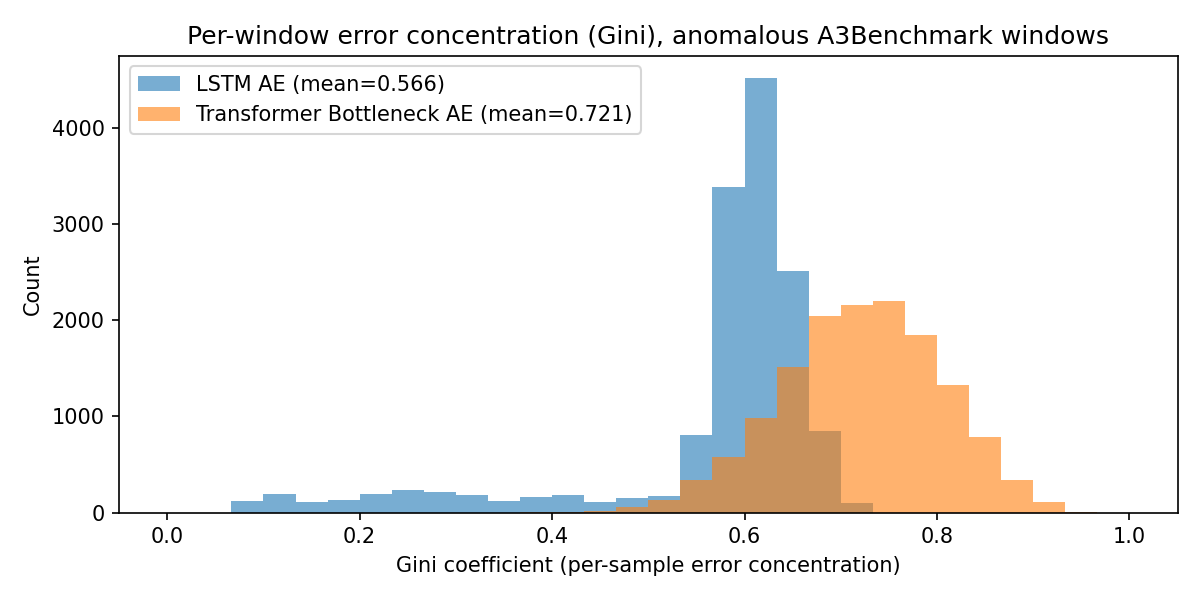
\includegraphics[width=0.55\textwidth]{../../data/explainability/yahoo_A3Benchmark_lstm_vs_transformer/5/gini_comparison.png}
\caption{Distribuția coeficienților Gini per fereastră, pe toate cele 14{,}449 ferestre A3 anormale. Distribuția Transformer-ului este unimodală și deplasată spre concentrare ridicată (Gini $>0.6$); distribuția LSTM Autoencoder-ului este bimodală, cu o majoritate grupată aproape de intervalul Transformer-ului, dar cu o populație secundară distinctă răspândită la valori Gini scăzute.}
\label{fig:explain-gini}
\end{figure}

Aceasta confirmă ipoteza inițială în mare: eroarea Transformer-ului este mai concentrată decât cea a LSTM Autoencoder-ului pe întreaga populație anormală, nu doar în exemplele arătate întâmplător de o hartă termică.
Distribuția din Figura~\ref{fig:explain-gini} arată însă că valorile Gini ale LSTM Autoencoder-ului sunt \emph{bimodale}, nu deplasate uniform în jos: o majoritate a ferestrelor sale ating o concentrare comparabilă cu a Transformer-ului (Gini $\approx 0.6$), dar o populație secundară distinctă rămâne la Gini scăzut ($<0.4$), cu eroarea cu adevărat difuzată. Mecanismul de distrugere a fazei afectează deci doar un subset specific de ferestre, iar această subpopulație -- nu o degradare generală -- explică scăderea AP-ului și ROC-AUC-ului agregat al LSTM Autoencoder-ului sub cel al Transformer-ului.





\section{Regimuri de Caracteristici Disjuncte: AE+Context vs.\ Temporal IForest}
\label{sec:explain-disjoint-regime}

Discuția despre CIC-IDS2017 din Capitolul~\ref{ch:results} propune combinarea AE+Context (puternic pe DDoS și PortScan) cu Temporal IForest (puternic pe clasele DoS lente și, cu rezerve, pe Heartbleed) într-un ansamblu, întrucât cele două ar trebui să opereze pe mulțimi de caracteristici disjuncte
-- caracteristici de context al gazdei versus o fereastră temporală de 16 fluxuri.

\paragraph{O scurtă introducere la SHAP.} SHAP (\emph{SHapley Additive exPlanations}) atribuie fiecărei caracteristici de intrare, per eșantion, o valoare care reflectă cât de mult a influențat aceasta ieșirea modelului: semnul arată direcția (spre normal sau anormal, convenție precizată separat pentru fiecare model mai jos, întrucât cele două nu coincid), iar magnitudinea arată contribuția relativă.
O \emph{diagramă beeswarm} (Figurile~\ref{fig:explain-temporal-beeswarm} și~\ref{fig:explain-ae-context-portscan-shap}) arată atribuirea pe un eșantion de puncte de test, un rând per caracteristică (ordonate descrescător după importanță), fiecare punct un eșantion poziționat orizontal după valoarea SHAP proprie și colorat după valoarea proprie a caracteristicii (albastru = mic, roșu = mare). Pentru definiția matematică și originea din teoria jocurilor cooperative: \parencite{lundberg2017unified}; pentru interpretarea grafurilor și construcția diagramelor de mai jos: documentația SHAP~\cite{shap_docs}.

Astfel, se presupune că: (1) dacă Temporal IForest exploatează cu adevărat structura dintre pașii temporali, scorul său per fereastră ar trebui să poarte informație despre eticheta \emph{ultimului} flux -- cel combinat cu scorul lui AE+Context -- nu doar despre dacă \emph{vreun} flux din fereastra de 16 este un atac, deci atribuirea sa SHAP nu ar trebui să se prăbușească pe acel flux final (altfel fereastra e doar decorativă); și (2) avantajul lui AE+Context pe propriile sale clase puternice provine din cele 9 caracteristici de context al gazdei, care ar trebui deci să apară printre caracteristicile cu cea mai mare medie $|\text{SHAP}|$.

O validare suplimentară -- că scorul lui Temporal IForest rămâne informativ și sub o etichetare mai strictă, per ultimul flux, nu doar sub eticheta permisivă \enquote{oricare-din-16} -- este detaliată în Anexa~\ref{ch:temporal-iforest-last-flow-validation}.



\subsection{Temporal IForest: Atribuire SHAP pe Toată Fereastra}
\label{sec:explain-temporal-window}

Temporal IForest este antrenat pe ferestre aplatizate de 16 fluxuri, deci valorile SHAP ale lui \texttt{TreeExplainer}~\parencite{lundberg2020local} pe intrarea aplatizată se descompun curat înapoi într-un cub (fereastră, pas temporal, caracteristică). Pentru fiecare din cele patru clase, SHAP a fost calculat pe 200 de ferestre;
magnitudinea atribuirii a fost sumată pe caracteristici per pas temporal, iar caracteristicile cu cea mai mare contribuție au fost reprezentate pe toți cei 16 pași temporali pentru a verifica dacă aceeași caracteristică poartă o atribuire cu semn consistent pe toată fereastra, nu doar aproape de final.

\begin{figure}[H]
\centering
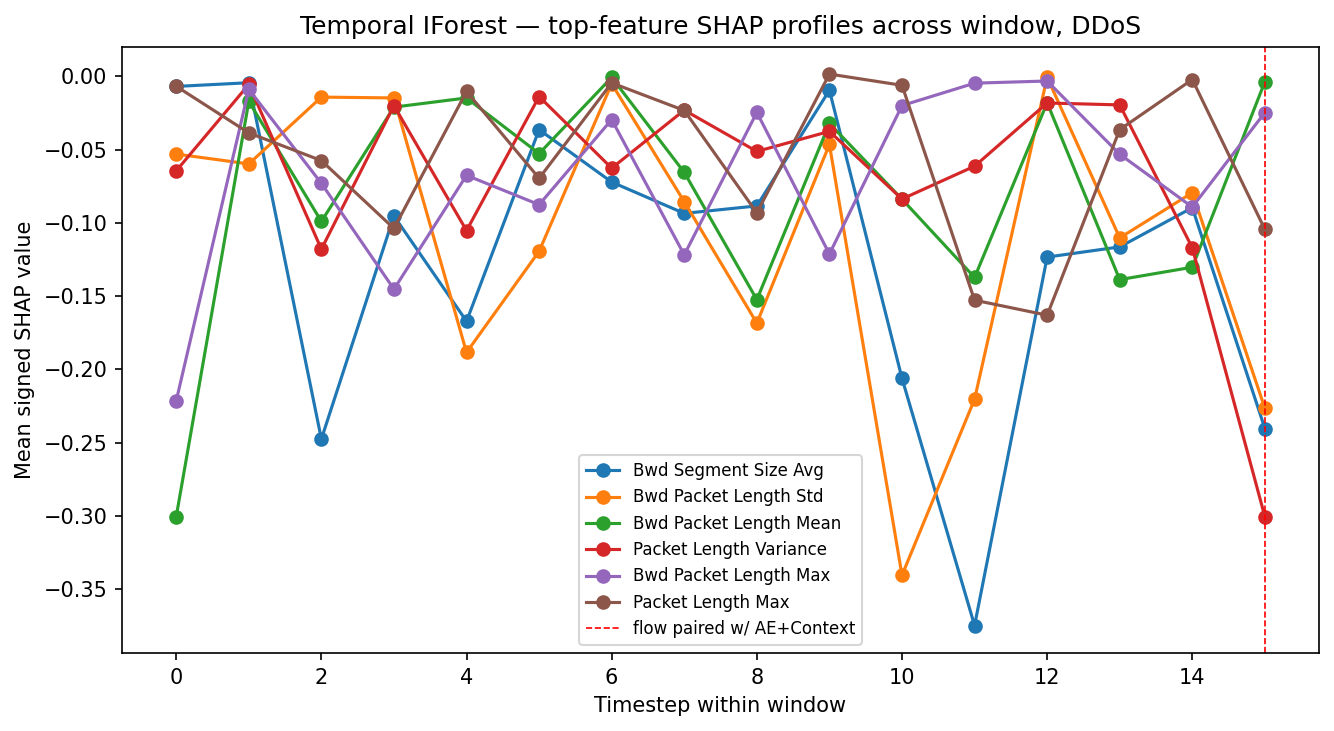
\includegraphics[width=0.42\textwidth,keepaspectratio]{../../data/explainability/cicids_temporal_shap/1/ddos_top_feature_profiles.png}%
\hspace{0.02\textwidth}%
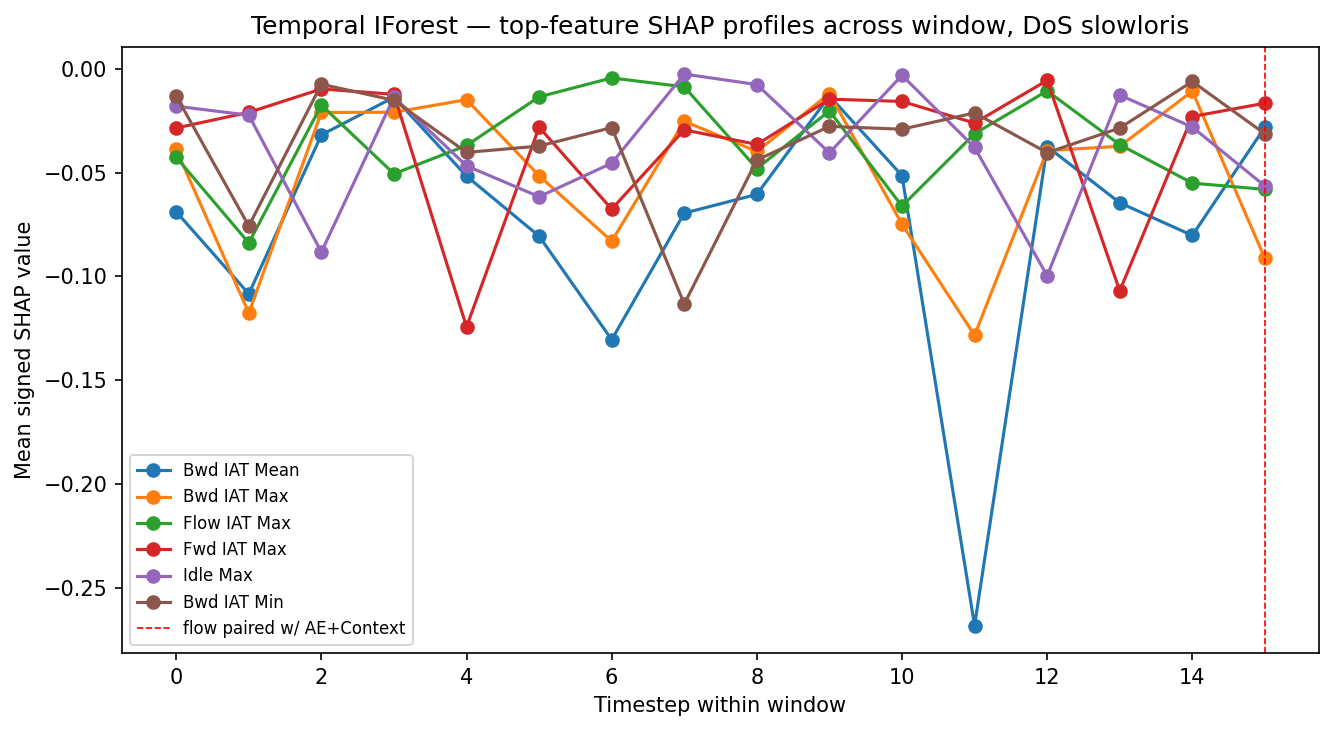
\includegraphics[width=0.42\textwidth,keepaspectratio]{../../data/explainability/cicids_temporal_shap/1/dos_slowloris_top_feature_profiles.png}

\caption{Temporal IForest -- valoarea medie SHAP per pas temporal pentru cele șase caracteristici cu cea mai mare atribuire, ferestre DDoS (stânga) și DoS slowloris (dreapta). Atribuirea e negativă (anormală) și recurentă pe majoritatea celor 16 pași, fără să se concentreze pe fluxul final (linia roșie punctată, cel combinat cu scorul AE+Context în ansamblul propus).}
\label{fig:explain-temporal-shap}
\end{figure}

Doi diagnostici suplimentari (Anexa~\ref{ch:temporal-shap-extra}) confirmă că ultimul pas temporal nu domină atribuirea (6--8\% din masa totală, aproape de referința uniformă de 6.25\%) și expun relația valoare-semn per caracteristică (monotonă pentru DoS slowloris, mai zgomotoasă pentru DDoS).
Caracteristicile principale se potrivesc cu mecanismul cunoscut al fiecărui atac: atribuirea DDoS/GoldenEye se concentrează pe lungimea pachetelor pe direcția inversă (\texttt{Bwd Packet Length Std/Mean/Max}), consistent cu un flux volumetric; atribuirea Slowhttptest/slowloris se concentrează pe timpul între sosiri (\texttt{Fwd/Bwd IAT Std/Max}), consistent cu comportamentul lent, de menținere a conexiunii -- confirmând ipoteza inițială.



\subsection{AE+Context: SHAP Dominat de Caracteristici de Context al Gazdei}

SHAP a fost calculat cu \texttt{GradientExplainer} pe eroarea de reconstrucție a lui AE+Context, pe câte 200 de eșantioane din PortScan și DDoS, iar cele 15 caracteristici cu cea mai mare medie $|\text{SHAP}|$ au fost clasate pentru fiecare clasă (diagrama sumară SHAP pentru PortScan este în Anexa~\ref{ch:temporal-shap-extra}, Figura~\ref{fig:explain-ae-context-portscan-shap}: \texttt{ctx\_min\_port\_cnt} domină printr-un cluster strâns, uniform pozitiv, bine separat de orice altă caracteristică).

\begin{center}
\begin{tabular}{@{}lcc@{}}
\toprule
 & Caracteristici de context în top 15 & Caracteristica principală (medie $|\text{SHAP}|$) \\
\midrule
PortScan & 8/15 & \texttt{ctx\_min\_port\_cnt} (0.324) \\
DDoS     & 7/15 & \texttt{ctx\_min\_port\_cnt} (0.234) \\
\bottomrule
\end{tabular}
\end{center}

Pentru ambele clase, \texttt{ctx\_min\_port\_cnt} și \texttt{ctx\_min\_flow\_cnt} domină cu aproximativ un ordin de mărime peste orice caracteristică de flux obișnuită, iar șase din cele nouă caracteristici de context apar în listele de top 15 ale ambelor clase (doar \texttt{ctx\_min\_port\_rate} lipsește din amândouă) -- confirmând premisa că avantajul lui AE+Context pe aceste clase este determinat aproape în întregime de dovezi de context al gazdei indisponibile lui Temporal IForest.



\subsection{Construirea Scorului Combinat}
\label{sec:explain-ensemble-build}

Realizarea ansamblului schițat în Capitolul~\ref{ch:results} necesită combinarea, pentru fiecare flux $f$, a scorului propriu al lui AE+Context cu scorul lui Temporal IForest pentru fereastra de 16 fluxuri care se \emph{încheie} la $f$. Cele două scoruri brute nu pot fi combinate direct (eroare de reconstrucție fără scală fixă vs.\ lungime medie de cale negată), deci e necesară o normalizare -- calculată doar pe scorurile de antrenare \emph{benigne} ale fiecărui model, niciodată pe date de test, pentru a evita scurgerea informației de anomalie în combinare.

Au fost testate două reguli: \textbf{votarea ponderată (soft voting)}, $s_{\text{soft}}(f) = w \cdot \hat{s}_{AE}(f) + (1-w) \cdot \hat{s}_{IF}(f)$, variind $w \in \{0.3, \dots, 0.7\}$; și \textbf{regula maximului}, $s_{\text{max}}(f) = \max(\hat{s}_{AE}(f), \hat{s}_{IF}(f))$ -- un combinator de tip OR, reflectând ideea că încrederea oricărui model, singură, ar trebui să fie suficientă.

Cele două scoruri au fost normalizate pe rang -- mapând fiecare scor de test la percentila sa în distribuția scorurilor proprii de antrenare benignă -- în locul standardizării $z$, care s-a dovedit o fundătură (normalizarea pe rang mărginește fiecare scor la $[0,1]$ indiferent de valoarea brută). Detalii despre realinierea scorurilor și eșecul standardizării $z$: Anexa~\ref{ch:ensemble-score-alignment}.

\subsection{Acoperire per Clasă vs.\ AP Agregat}
\label{sec:explain-ensemble-results}

\begin{center}
\begin{tabular}{@{}lccccc@{}}
\toprule
 & DDoS & PortScan & GoldenEye & Slowhttptest & slowloris \\
\midrule
AE+Context singur         & 0.882 & \textbf{0.924} & 0.292 & 0.013 & 0.025 \\
Temporal IForest singur   & \textbf{0.956} & 0.123 & 0.611 & 0.578 & 0.560 \\
Regula maximului (rang)   & 0.882 & 0.923 & 0.292 & 0.060 & 0.083 \\
Votare ponderată $w=0.4$ (rang) & 0.977 & 0.228 & \textbf{0.801} & \textbf{0.205} & \textbf{0.319} \\
Votare ponderată $w=0.7$ (rang) & 0.977 & 0.358 & 0.821 & 0.140 & 0.245 \\
\bottomrule
\end{tabular}
\end{center}

AP-ul agregat \emph{favorizează} de fapt variantele care se schimbă cel mai puțin: regula maximului (0.943) și AE+Context singur (0.941) depășesc votarea ponderată $w=0.4$ (0.841), pur și simplu pentru că DDoS și PortScan totalizează peste 250{,}000 din cele $\sim$434{,}000 de fluxuri pozitive, față de doar 13{,}000 pentru GoldenEye, Slowhttptest și slowloris împreună.

Nicio regulă nu e un câștig gratuit, dar votarea ponderată pare alegerea mai pertinentă pentru un ansamblu motivat de acoperire: clasa sa cea mai \emph{slabă} (0.205, Slowhttptest, la $w=0.4$) depășește propriile clase cele mai slabe ale ambelor modele singure -- 0.013 (AE+Context) și 0.123 (Temporal IForest) -- ceva ce niciun model singur sau regula maximului nu realizează. E o realizare autentică, deși parțială, a ideii de ansamblu din Capitolul~\ref{ch:results}: votarea ponderată pe rang lărgește pragul minim de acoperire, cu costul detecției PortScan.

\chapter{Concluzii}
\label{ch:concluzii}

Întrebarea formulată în Capitolul~\ref{ch:introducere} a fost în ce măsură modul în care un model reprezintă structura latentă a datelor \enquote{normale} determină tipurile de anomalii pe care le poate detecta. Rezultatele din Capitolul~\ref{ch:results}, confirmate și nuanțate în Capitolul~\ref{ch:explainability}, dau un răspuns afirmativ: aceeași paradigmă produce rezultate diferite pe seturi de date diferite nu pentru că modelul ar fi mai bun sau mai slab în sine, ci pentru că presupunerea lui despre normalitate se potrivește sau nu structurii reale a anomaliei căutate.

Cele două ipoteze din \S\ref{sec:expected-behaviour} se confirmă, dar nu necondiționat. Prima -- structura temporală avantajează datele secvențiale -- se confirmă pe Yahoo A3/A4 (paradigma predictivă domină), dar se inversează pe Setul A (secvență artificială) și e depășită de contextul de gazdă la CIC-IDS2017. A doua -- paradigme complementare, combinate, îmbunătățesc performanța -- e confirmată de studiul din \S\ref{sec:explain-disjoint-regime}: AE+Context și Temporal IForest exploatează evidențe disjuncte, iar votarea ponderată extinde acoperirea pe clase altfel nedetectate, cu costul unui AP agregat mai mic -- nuanțând, nu infirmând, ipoteza inițială.

Limitările deschid două direcții: testarea sistematică a celorlalte presupuneri din Capitolul~\ref{ch:results} și extinderea studiului de ansamblu din \S\ref{sec:explain-ensemble-build} la Seturile A și B, cu reguli de combinare mai sofisticate.

\enlargethispage{\baselineskip}

\cleardoublepage
\appendix
\renewcommand{\thechapter}{\arabic{chapter}}
\renewcommand{\appendixtocname}{Anexe}
\addappheadtotoc
\chapter{Detalii Suplimentare de Preprocesare}
\label{sec:preprocessing-details}

Această anexă completează Secțiunea~\ref{sec:preprocessing} cu pașii exacți ai fiecărui pipeline de preprocesare.

\section{Preprocesare Tabelară (Credit Card)}

\begin{enumerate}
  \item \texttt{Time} este eliminat (nu reprezintă informație semnificativă, întrucât este doar timpul de la prima tranzacție din setul de date).
  \item Rândurile sunt împărțite pe clase: toate rândurile benigne (\texttt{Class=0}) sunt reunite, apoi împărțite 80/20 în antrenare și test-benign. Setul de antrenare este partiția de 80\%, conținând doar rânduri benigne ($\sim$227{,}451 rânduri).
  \item Setul de testare este format din restul de 20\% rânduri benigne, plus \emph{toate} cele 492 de rânduri de fraudă.
  \item Scalarea este asimetrică, pe grupuri de caracteristici: \texttt{V1--V28} trec \textbf{nescalate} implicit (\texttt{V\_SCALING = 'none'} -- întrucât acestea sunt deja caracteristici PCA), cu \texttt{'standard'} încercat de asemenea în unele rulări, fără o diferență reală între modele. \texttt{Amount} este scalat independent cu un \texttt{RobustScaler} (bazat pe mediană/IQR), ales pentru robustețea sa la coada dreaptă accentuată, urmând același raționament ca notebook-ul exploratoriu citat în \S\ref{ch:preliminarii}.
\end{enumerate}

\section{Crearea de Ferestre pentru Serii de Timp (Yahoo S5)}

\begin{enumerate}
  \item Fiecare serie este împărțită 70/30 de-a lungul axei temporale (\texttt{TRAIN\_FRAC=0.70}) -- o împărțire temporală și nu o amestecare aleatoare. Nu vrem ca vreo informație din viitor să se scurgă în antrenare.
  \item Un \texttt{MinMaxScaler} este potrivit \emph{per serie}, folosind doar punctele neanormale din partiția de antrenare a acelei serii, apoi aplicat atât partiției de antrenare, cât și celei de testare ale aceleiași serii.
  \item Se aplică o fereastră glisantă de lungime \texttt{WINDOW=64}: pas 4 pentru ferestrele de antrenare (subeșantionate, păstrându-se pentru antrenare doar ferestrele complet normale) și pas 1 pentru ferestrele de testare (dens -- este evaluată fiecare poziție posibilă a ferestrei).
  \item Eticheta unei ferestre urmează regula \enquote{oricare}: pozitivă dacă cel puțin unul dintre cei 64 de pași de timp este anormal. Aceasta este totuși o sursă de \enquote{estompare} a etichetelor -- de exemplu, pe A1, o rată de anomalii la nivel de punct de $1.76\%$ devine o rată la nivel de fereastră de $\sim$17--18\%, întrucât un singur punct anormal contaminează până la 64 de ferestre suprapuse. O fereastră mai mică ar reduce această estompare, lucru care ar putea merita încercat în viitor.
  \item Ferestrele din toate seriile unui benchmark (reamintesc că fiecare benchmark este alcătuit din mai multe serii univariate) sunt reunite în array-uri unice.
\end{enumerate}

\paragraph{Comparație cu DeepAnt.} DeepAnt~\parencite{munir2019deepant} a fost folosit ca referință pentru evaluarea unui predictor neural al pasului următor pe Yahoo S5, deși mai multe alegeri metodologice diferă de cele ale acestui proiect:

\begin{itemize}
  \item \textbf{Predicție many-to-one, nu many-to-many.} Predictorul propus de DeepAnt este o rețea convoluțională; varianta LSTM raportată de aceștia ca referință de comparație (două straturi suprapuse, de câte 32 de unități) este mai îngustă și mai puțin adâncă decât LSTM-ul de 64 de unități folosit aici pentru LSTM Predictiv. Mai important, ambele prezic doar un singur pas de timp următor dintr-o fereastră (many-to-one), în loc de fiecare pas $t{+}1$ din $0..t$ simultan, așa cum fac modelele predictive ale acestui proiect (\S\ref{ch:preliminarii}).
  \item \textbf{Antrenare per serie vs.\ antrenare reunită.} DeepAnt antrenează și evaluează un model separat pentru fiecare serie de timp individuală (o împărțire 40/60 antrenare/test per serie, scorul F calculat per serie și apoi mediat per sub-benchmark), ceea ce permite fiecărui model să se specializeze pe o singură frecvență. Acest proiect reunește în schimb ferestrele din toate cele $\sim$100 de serii ale unui benchmark într-un singur model comun, antrenat pe o împărțire 70/30 -- în principal din motive de simplitate a implementării.
\end{itemize}

\section{Preprocesarea Fluxurilor de Rețea (CIC-IDS2017)}

Există trei implementări pentru acest set de date, toate având la bază aceiași pași de curățare (eliminarea \texttt{Flow ID}/\texttt{Src IP}/\texttt{Dst IP}/\texttt{Timestamp}/\texttt{Src Port}; codificare one-hot pentru \texttt{Protocol}; înlocuirea \texttt{Inf} cu \texttt{NaN}; imputare cu mediana, calculată pe setul de antrenare; eliminarea coloanelor cu varianță zero, măsurată pe setul de antrenare; \texttt{MinMaxScaler} potrivit doar pe setul de antrenare), dar diferind prin unitatea de observație:

\paragraph{Plat} Un rând = un flux. Setul de antrenare este format din toate fluxurile benigne din ziua de luni (371{,}749 rânduri); setul de testare conține toate fluxurile benigne de marți--vineri, plus toate fluxurile de atac reale (fluxurile \texttt{-- Attempted}, adică atacuri fără încărcătură observată, sunt excluse complet). Filtrarea coloanelor cu varianță zero pe datele de luni elimină cele trei coloane de flag URG, rămânând 77 din cele 80 de caracteristici originale.

\paragraph{Temporal} Un rând = o fereastră de \texttt{WINDOW=16} fluxuri consecutive de la aceeași adresă IP sursă, sortate după timestamp.
Această alegere de grupare -- după IP sursă, nu după sesiunea individuală de flux (identificată printr-un 5-tuplu: IP sursă, IP destinație, port sursă, port destinație și protocol -- cei cinci identificatori pe baza cărora CICFlowMeter definește o conexiune individuală) -- corespunde cheii de grupare folosite și pentru calculul caracteristicilor de context de gazdă de mai jos.
Ambele pipeline-uri tratează \enquote{o entitate} drept fluxul de activitate ordonat al unei gazde sursă, nu o conexiune 5-tuplu, întrucât comportamentul la nivel de gazdă (multe conexiuni scurte, în rafală) caracterizează atacuri precum PortScan sau DoS, mai degrabă decât structura internă a unei singure conexiuni. Împărțirea este pe zile (luni antrenare, marți--vineri testare), din același motiv ca la pipeline-ul plat.

\paragraph{Context de gazdă} Aceeași curățare plată, per flux, ca mai sus, dar fiecare flux este suplimentat cu 9 caracteristici construite, calculate dintr-o fereastră temporală glisantă de 60 de secunde, per IP gazdă: numărul de fluxuri, numărul de porturi unice, rata de diversitate a porturilor, un indicator de port nou, precum și asimetria sursă/destinație a fiecăreia. Acestea sunt calculate cauzal (doar din activitatea \emph{anterioară} fluxului curent) și nu necesită etichete de atac, urmând adaptarea nesupervizată a lui \textcite{raskovalov2024nids}. Numărul final de caracteristici: $77 + 9 = 86$. Această variantă a fost introdusă special pentru a rezolva o slăbiciune comună pipeline-urilor plat și temporal, pe clasa de atac PortScan (vezi \S\ref{ch:results}).

\chapter{Alegeri legate de Hiperparametri și Antrenare}
\label{sec:architecture}

Două decizii principale se aplică uniform pentru toate modelele și seturile de date:

\begin{itemize}
  \item \textbf{Optimizator.} Toate rețelele neuronale sunt antrenate cu Adam, la o rată de învățare fixă de $10^{-3}$, uniform pentru fiecare model și set de date.
  \item \textbf{Fără căutare de hiperparametri.} Dacă un model a avut performanțe neașteptat de slabe, rata sa de învățare a fost verificată suplimentar cu $\{10^{-4}, 10^{-3}, 3\times10^{-3}\}$ înainte de a trage vreo concluzie din acel rezultat.
  \item \textbf{Partiție de validare doar pentru monitorizare.} Fiecare rețea neuronală reține aleator 10\% din datele de antrenare exclusiv pentru a trasa o curbă de pierdere (\emph{loss}) de antrenare/validare per rulare, ca verificare că antrenarea decurge corect. Această partiție nu este niciodată folosită pentru oprire timpurie (\emph{early stopping}) sau selecția modelului: antrenarea rulează întotdeauna pentru numărul fix de epoci de mai jos, iar rezultatele raportate pe setul de testare folosesc ponderile modelului din epoca finală.
\end{itemize}

\section{Isolation Forest}

\begin{center}
\begin{tabular}{@{}lllll@{}}
\toprule
 & CIC flat & CIC context & Yahoo & Credit card \\
\midrule
N\_ESTIMATORS & 150 & 150 & 150 & 150 \\
MAX\_SAMPLES & 300{,}000 & 300{,}000 & $\min(n, 50{,}000)$ & 200{,}000 \\
Dimensiunea setului de antrenare & $\sim$371k & $\sim$371k & câteva mii & $\sim$227k \\
\% din antrenare folosit & $\sim$81\% & $\sim$81\% & $\sim$100\% & $\sim$88\% \\
RANDOM\_SEED & 123 & 123 & 123 & 123 \\
\bottomrule
\end{tabular}
\end{center}

\texttt{MAX\_SAMPLES} este singura diferență semnificativă și este setat cât mai ridicat posibil, practic, pentru fiecare set de date (acuratețea crește odată cu mai multe eșantioane per arbore, cu randamente descrescânde;
problema de \enquote{swamping} al arborilor nu apare aici, întrucât datele de antrenare sunt întotdeauna exclusiv benigne). Plafonul de 50.000 pentru Yahoo nu este atins niciodată în practică și este păstrat doar ca limită de siguranță.

\section{One-Class SVM}

\begin{center}
\begin{tabular}{@{}lllll@{}}
\toprule
 & CIC flat & CIC context & Yahoo & Credit card \\
\midrule
NU & 0.01 & 0.01 & 0.01 & 0.01 \\
KERNEL & rbf & rbf & rbf & rbf \\
GAMMA & scale & scale & scale & scale \\
SUBSAMPLE & 50{,}000 & 50{,}000 & niciunul (complet) & niciunul (complet) \\
\% din antrenare folosit & $\sim$13.5\% & $\sim$13.5\% & $\sim$100\% & $\sim$100\% \\
\bottomrule
\end{tabular}
\end{center}

Toți parametrii kernel/nu sunt uniformi pe seturile de date. Subeșantionarea este aplicată doar acolo unde setul de antrenare este suficient de mare încât un OC-SVM pe toate datele ar deveni mult prea lent; credit card ($\sim$227k rânduri) a fost antrenat pe tot setul, fără subeșantionare.

\section{Autoencoder Feedforward (MLP)}

\begin{center}
\begin{tabular}{@{}lllll@{}}
\toprule
 & CIC flat & CIC context & Yahoo & Credit card \\
\midrule
Dimensiune intrare & 77 & 86 & 64 (fereastră aplatizată) & $\sim$30 (PCA) \\
Dimensiuni ascunse & [64, 32, 16] & [64, 32, 16] & [32, 16] & [16, 8] \\
Raport bottleneck & 0.21 & 0.19 & 0.25 & $\sim$0.27 \\
Activare finală & Sigmoid & Sigmoid & Linear & Linear \\
\bottomrule
\end{tabular}
\end{center}

Lățimile straturilor sunt scalate în funcție de dimensiunea intrării, astfel încât raportul de compresie al bottleneck-ului să rămână aproximativ constant ($\sim$0.20--0.27) pe toate seturile de date. Activarea finală diferă întrucât CIC folosește \texttt{MinMaxScaler} (mărginit la $[0,1]$, potrivit pentru o ieșire sigmoid), în timp ce Yahoo și credit card folosesc scalere nemărginite (ieșire liniară).

\section{LSTM Predictiv}

\begin{center}
\begin{tabular}{@{}llll@{}}
\toprule
 & CIC & Yahoo & Credit card \\
\midrule
INPUT\_SIZE & 77 & 1 & 1 \\
HIDDEN\_DIM & 128 & 64 & 64 \\
NUM\_LAYERS & 1 & 1 & 1 \\
EPOCHS & 20 & 20 & 50 \\
BATCH\_SIZE & 256 & 256 & 512 \\
\bottomrule
\end{tabular}
\end{center}

\texttt{HIDDEN\_DIM} este scalat în funcție de dimensiunea intrării pentru CIC (o extindere de $\sim$1.66$\times$ față de cele 77 de caracteristici de intrare); ambele seturi de date univariate folosesc 64, o capacitate suficientă pentru un semnal scalar. Credit card folosește mai multe epoci (50) întrucât curba sa de pierdere continuă să scadă și după epoca 30 -- probabil o consecință directă a tratării celor 29 de caracteristici PCA netemporale ca pseudo-secvență, ceea ce face optimizarea mai zgomotoasă decât pe date cu adevărat temporale. CIC și Yahoo converg până la epoca $\sim$5, deci 20 de epoci este deja o alegere conservatoare pentru acestea.

\section{Autoencoder LSTM}

\begin{center}
\begin{tabular}{llll}
\toprule
 & CIC & Yahoo & Credit card \\
\midrule
INPUT\_SIZE & 77 & 1 & 1 \\
HIDDEN\_DIM & 128 & 64 & 64 \\
NUM\_LAYERS & 1 & 1 & 1 \\
EPOCHS & 50 & 30 & 50 \\
BATCH\_SIZE & 256 & 256 & 512 \\
\bottomrule
\end{tabular}
\end{center}

Atât CIC, cât și credit card au necesitat 50 de epoci pentru a atinge un platou; Yahoo converge până la epoca $\sim$5, deci 30 este deja generos.

\section{Detalii de Arhitectură: Autoencodere Bazate pe Transformer}
\label{sec:transformer-architecture-details}

Această secțiune completează \S\ref{sec:paradigms} cu detalii suplimentare despre cele două variante de transformer.

\textbf{Bottleneck Transformer Autoencoder} -- bazat pe reconstrucție. Fiecare caracteristică/pas de timp de intrare este proiectat(ă) într-un token de dimensiune $\texttt{D\_MODEL}$ și trecut(ă) prin encoderul transformer cu auto-atenție completă (non-cauzală), astfel încât fiecare poziție poate atenționa liber orice altă poziție. Reprezentările rezultate per poziție sunt apoi \emph{mediate global} (\emph{global-average-pooled}) de-a lungul secvenței într-un singur vector de dimensiune $\texttt{D\_MODEL}$, comprimat printr-un strat liniar la un \texttt{LATENT\_DIM} strict mai mic, apoi extins înapoi printr-un al doilea strat liniar la forma completă a secvenței aplatizate.
Acest pas de comprimare-extindere este bottleneck-ul explicit de informație (analog stării ascunse finale din Autoencoder LSTM) care împiedică mecanismul de atenție să copieze pur și simplu intrarea în ieșire.
Scor de anomalie: MSE per eșantion între intrare și reconstrucție, pe toate pozițiile deodată -- întreaga secvență reconstruită este produsă printr-o singură trecere prin rețea, nu pas cu pas ca la un decoder recurent.

\textbf{Causal Transformer} -- predictiv-temporal, echivalentul bazat pe atenție al LSTM Predictiv. Este folosită aceeași structură de encoder, dar cu o mască de atenție cauzală (triunghiulară superior) aplicată, astfel încât poziția $t$ poate atenționa doar pozițiile $0..t$; modelul este antrenat cu același obiectiv de predicție a pasului următor ca LSTM Predictiv, fără bottleneck de comprimare.
Scor de anomalie: MSE per eșantion între valorile prezise și cele reale ale pasului următor.

\paragraph{De ce un singur \texttt{TransformerEncoder}.} Ambele variante folosesc deliberat un singur encoder. Costul de antrenare și inferență crește odată cu numărul de straturi de atenție, pe toate seturile de date și modelele, iar un design de tip encoder-only păstrează acest cost, împreună cu numărul de parametri antrenabili, la aproximativ jumătate din ce ar necesita un model echivalent encoder-decoder, fără a sacrifica abilitatea de a face fie comprimare-și-reconstrucție, fie predicție cauzală.

\section{Bottleneck Transformer Autoencoder}

\begin{center}
\begin{tabular}{llll}
\toprule
 & CIC & Yahoo & Credit card \\
\midrule
D\_MODEL & 64 & 64 & 64 \\
NHEAD & 4 & 4 & 4 \\
NUM\_LAYERS & 2 & 2 & 2 \\
DIM\_FF & 256 & 256 & 256 \\
LATENT\_DIM & 32 & 32 & 32 \\
EPOCHS & 50 & 20 & 20 \\
BATCH\_SIZE & 256 & 256 & 512 \\
\bottomrule
\end{tabular}
\end{center}

\texttt{LATENT\_DIM=32} oferă o compresie uniformă de 50\% față de \texttt{D\_MODEL=64}, pe toate cele trei seturi de date.

\section{Causal Transformer}

\begin{center}
\begin{tabular}{lll}
\toprule
 & CIC & Yahoo \\
\midrule
D\_MODEL & 64 & 64 \\
NHEAD & 4 & 4 \\
NUM\_LAYERS & 2 & 2 \\
DIM\_FF & 256 & 256 \\
DROPOUT & 0.1 & 0.1 \\
EPOCHS & 30 & 30 \\
BATCH\_SIZE & 256 & 256 \\
\bottomrule
\end{tabular}
\end{center}



\chapter{Protocolul de Evaluare: Metrici și Rezultate Complete}
\label{sec:eval-metrics}

\section{Metrici Raportate}

Fiecare rulare produce un raport text care conține toate metricile din Tabelul~\ref{tab:eval-metrics-def}. Capitolul de Rezultate raportează doar un subset dintre acestea (de obicei ROC-AUC, Precizia Medie, și, unde este relevant, Acuratețea Echilibrată și F1), ales pentru a nu aglomera tabelele de comparație; setul complet, per model și per set de date, este prezentat în \S\ref{sec:eval-full-cc}--\S\ref{sec:eval-full-cic}.

\begin{table}[H]
\centering
\begin{tabular}{@{}p{4cm}p{9.5cm}@{}}
\toprule
Metrică & Note \\
\midrule
Precizie / Recall / F1 (per clasă) & Prin \texttt{sklearn.classification\_report}, raportate atât pentru clasa normală, cât și pentru clasa anomalie, plus acuratețea și mediile macro/ponderate. \\
ROC-AUC & Raportat pentru completitudine / comparabilitate cu literatura anterioară; nu este metrica principală de clasificare în condiții de dezechilibru de clase. \\
Precizie Medie (PR-AUC) & Independentă de prag; alegerea standard în condiții de dezechilibru sever de clase, întrucât ROC-AUC poate părea înșelător de bun atunci când exemplele negative depășesc masiv numărul celor pozitive. \\
Acuratețe Echilibrată & $\frac{1}{2}(\text{sensibilitate} + \text{specificitate})$ la pragul de operare selectat. \\
F1 (clasa pozitivă/atac) & La pragul de operare selectat. \\
Numărători din matricea de confuzie & TP/TN/FP/FN brute, la pragul selectat. \\
\bottomrule
\end{tabular}
\caption{Metrici raportate de fiecare rulare de evaluare.}
\label{tab:eval-metrics-def}
\end{table}

\paragraph{Notă privind consistența numerelor.} Tabelele~\ref{tab:eval-full-cc}--\ref{tab:eval-full-cic} de mai jos completează Capitolul~\ref{ch:results} cu detaliul complet (precizie/recall pe clasa pozitivă, matrice de confuzie) pentru fiecare model. 
Coloanele ROC-AUC / Precizie Medie / Acuratețe Echilibrată / F1 reproduc exact valorile deja publicate în Capitolul~\ref{ch:results}, pentru consistență. Pentru un număr de modele -- în special pe CIC-IDS2017, unde reevaluări ulterioare au schimbat scorurile -- nu toate metricile au mai fost calculate. În aceste cazuri, rândul din tabel afișează doar metricile agregate deja publicate.

\section{Rezultate Complete -- Credit Card Fraud Detection}
\label{sec:eval-full-cc}

\begin{table}[H]
\centering
\resizebox{\textwidth}{!}{%
\begin{tabular}{@{}lcccccccccc@{}}
\toprule
Model & Precizie (fraudă) & Recall (fraudă) & F1 (fraudă) & ROC-AUC & Precizie Medie & Acuratețe Echilibrată & TP & TN & FP & FN \\
\midrule
MLP Autoencoder           & 0.6205 & 0.8008 & 0.6992 & 0.9649 & 0.7105 & 0.8983 & 394 & 56622 & 241 & 98 \\
Isolation Forest          & 0.5000 & 0.7724 & 0.6070 & 0.9587 & 0.6725 & 0.8828 & 380 & 56483 & 380 & 112 \\
LSTM Autoencoder          & 0.6904 & 0.7886 & 0.7362 & 0.9476 & 0.6223 & 0.8928 & 388 & 56689 & 174 & 104 \\
OC-SVM                    & 0.5501 & 0.7805 & 0.6454 & 0.9354 & 0.5959 & 0.8875 & 384 & 56549 & 314 & 108 \\
Transformer Bottleneck AE & 0.5073 & 0.7764 & 0.6137 & 0.9583 & 0.5947 & 0.8849 & 382 & 56492 & 371 & 110 \\
Predictive LSTM           & 0.3992 & 0.7642 & 0.5244 & 0.9581 & 0.5190 & 0.8771 & 376 & 56297 & 566 & 116 \\
\bottomrule
\end{tabular}%
}
\caption{Credit Card Fraud Detection -- toate metricile raportate, pentru toate cele șase modele evaluate.}
\label{tab:eval-full-cc}
\end{table}

\section{Rezultate Complete -- Yahoo Webscope S5}
\label{sec:eval-full-yahoo}

\begin{table}[H]
\centering
\resizebox{\textwidth}{!}{%
\begin{tabular}{@{}lcccccccccc@{}}
\toprule
Model & Precizie (poz.) & Recall (poz.) & F1 (poz.) & ROC-AUC & Precizie Medie & Acuratețe Echilibrată & TP & TN & FP & FN \\
\midrule
\multicolumn{11}{@{}l}{\textbf{A1 -- anomalii punctuale}} \\
MLP Autoencoder  & -- & -- & -- & 0.792 & 0.611 & -- & -- & -- & -- & -- \\
LSTM Autoencoder & 0.2944 & 0.7904 & 0.4290 & 0.794 & 0.600 & 0.6916 & 852 & 2974 & 2042 & 226 \\
OC-SVM           & 0.5183 & 0.5909 & 0.5522 & 0.776 & 0.595 & 0.7364 & 637 & 4424 & 592 & 441 \\
LSTM Predictiv   & 0.2988 & 0.8016 & 0.4354 & 0.789 & 0.588 & 0.6988 & 3442 & 11912 & 8076 & 852 \\
Isolation Forest & 0.2439 & 0.8646 & 0.3805 & 0.765 & 0.511 & 0.6443 & 932 & 2127 & 2889 & 146 \\
\midrule
\multicolumn{11}{@{}l}{\textbf{A3 -- anomalii contextuale/sezoniere}} \\
LSTM Predictiv             & -- & -- & -- & 0.868 & 0.812 & -- & -- & -- & -- & -- \\
Transformer Bottleneck AE  & -- & -- & -- & 0.762 & 0.663 & -- & -- & -- & -- & -- \\
Causal Transformer         & -- & -- & -- & 0.738 & 0.623 & -- & -- & -- & -- & -- \\
MLP Autoencoder            & 0.4247 & 0.9540 & 0.5878 & 0.765 & 0.507 & 0.6622 & 13785 & 10981 & 18670 & 664 \\
LSTM Autoencoder           & 0.3278 & 1.0000 & 0.4937 & 0.566 & 0.392 & 0.5003 & 14449 & 20 & 29631 & 0 \\
OC-SVM                     & 0.3285 & 0.9996 & 0.4945 & 0.584 & 0.376 & 0.5020 & 14443 & 128 & 29523 & 6 \\
Isolation Forest           & 0.3301 & 0.9960 & 0.4959 & 0.511 & 0.331 & 0.5055 & 14391 & 447 & 29204 & 58 \\
\midrule
\multicolumn{11}{@{}l}{\textbf{A4 -- schimbări de nivel}} \\
LSTM Predictiv             & 0.3975 & 0.7951 & 0.5300 & 0.745 & 0.505 & 0.6864 & 9098 & 18868 & 13789 & 2345 \\
Causal Transformer         & 0.3092 & 0.9098 & 0.4616 & 0.695 & 0.436 & 0.5988 & 10411 & 9401 & 23256 & 1032 \\
MLP Autoencoder            & -- & -- & -- & 0.719 & 0.402 & -- & -- & -- & -- & -- \\
Transformer Bottleneck AE  & 0.2625 & 0.9959 & 0.4155 & 0.655 & 0.404 & 0.5077 & 11396 & 636 & 32021 & 47 \\
Isolation Forest           & 0.2595 & 1.0000 & 0.4121 & 0.498 & 0.268 & 0.5001 & 11443 & 6 & 32651 & 0 \\
OC-SVM                     & 0.2603 & 1.0000 & 0.4131 & 0.519 & 0.265 & 0.5021 & 11443 & 139 & 32518 & 0 \\
LSTM Autoencoder           & 0.2644 & 0.9979 & 0.4181 & 0.502 & 0.252 & 0.5127 & 11419 & 895 & 31762 & 24 \\
\bottomrule
\end{tabular}%
}
\caption{Yahoo Webscope S5 -- toate metricile raportate, pe benchmark (A1, A3, A4), ordonate ca în tabelele din Capitolul~\ref{ch:results}.}
\label{tab:eval-full-yahoo}
\end{table}

\section{Rezultate Complete -- CIC-IDS2017}
\label{sec:eval-full-cic}

Compoziția pe clase de atac a setului de test temporal (analoagă Tabelului~\ref{tab:cic-composition} din Capitolul~\ref{ch:results} pentru setul flat/context) este detaliată separat, în Capitolul~\ref{ch:cic-composition-temporal}.

\begin{table}[H]
\centering
\resizebox{\textwidth}{!}{%
\begin{tabular}{@{}llcccccccccc@{}}
\toprule
Model & Set de caracteristici & Precizie (atac) & Recall (atac) & F1 (atac) & ROC-AUC & Precizie Medie & Acuratețe Echilibrată & TP & TN & FP & FN \\
\midrule
MLP Autoencoder            & Context  & -- & -- & -- & 0.9860 & 0.9487 & 0.9548 & -- & -- & -- & -- \\
OC-SVM                     & Context  & 0.8965 & 0.9509 & 0.9229 & 0.9745 & 0.9396 & 0.9569 & 412650 & 1238310 & 47634 & 21327 \\
Isolation Forest           & Context  & -- & -- & -- & 0.9785 & 0.9328 & 0.9270 & -- & -- & -- & -- \\
LSTM Autoencoder           & Temporal & 0.4752 & 0.9126 & 0.6249 & 0.8976 & 0.7955 & 0.7846 & 398793 & 842158 & 440453 & 38212 \\
MLP Autoencoder            & Flat     & -- & -- & -- & 0.9189 & 0.7921 & 0.8022 & -- & -- & -- & -- \\
Isolation Forest           & Flat     & -- & -- & -- & 0.9049 & 0.7612 & 0.8228 & -- & -- & -- & -- \\
OC-SVM                     & Temporal & 0.4214 & 0.9770 & 0.5888 & 0.8629 & 0.7816 & 0.7600 & 426967 & 696384 & 586227 & 10038 \\
MLP Autoencoder            & Temporal & -- & -- & -- & 0.8831 & 0.7509 & 0.7734 & -- & -- & -- & -- \\
Isolation Forest           & Temporal & 0.3577 & 0.9487 & 0.5195 & 0.8438 & 0.7604 & 0.6841 & 414606 & 538115 & 744496 & 22399 \\
OC-SVM                     & Flat     & 0.3045 & 0.9778 & 0.4644 & 0.7336 & 0.6845 & 0.6121 & 424338 & 316815 & 969129 & 9639 \\
Bottleneck Transformer AE  & Temporal & -- & -- & -- & 0.8077 & 0.6539 & 0.7059 & -- & -- & -- & -- \\
Causal Transformer         & Temporal & -- & -- & -- & 0.7099 & 0.5449 & 0.5520 & -- & -- & -- & -- \\
Predictive LSTM            & Temporal & -- & -- & -- & 0.6126 & 0.4472 & 0.5475 & -- & -- & -- & -- \\
\bottomrule
\end{tabular}%
}
\caption{CIC-IDS2017 -- toate metricile raportate, pentru toate cele treisprezece combinații model/set-de-caracteristici, ordonate ca în Tabelul din \S\ref{ch:results}.}
\label{tab:eval-full-cic}
\end{table}



\section{Detaliere Suplimentară pe Tip de Atac -- Modele cu Context}
\label{sec:cic-per-attack-appendix}

Această secțiune completează \S\ref{sec:cic-per-attack} cu Precizia Medie pe clasă de atac, pentru cele trei modele cu context, și cu detaliul răspunsului per model la cele trei clase DoS la nivel de aplicație (GoldenEye, Slowhttptest, slowloris), unde familia de context nu răspunde uniform.

\begin{table}[H]
\centering
\resizebox{\textwidth}{!}{%
\begin{tabular}{@{}lrlll@{}}
\toprule
Clasă de atac & $n$ & IForest+Ctx & OC-SVM+Ctx & AE+Ctx \\
\midrule
DDoS                & 95{,}000  & 0.982          & \textbf{0.998} & 0.994          \\
PortScan             & 159{,}000 & 0.601          & 0.820          & \textbf{0.842} \\
DoS GoldenEye        & 7{,}500   & \textbf{0.655} & 0.215          & 0.220          \\
DoS slowloris        & 4{,}000   & \textbf{0.190} & 0.012          & 0.025          \\
DoS Slowhttptest     & 1{,}700   & \textbf{0.112} & 0.007          & 0.013          \\
Heartbleed           & 11        & \textbf{0.093} & 0.001          & 0.000          \\
Infiltration         & 32        & \multicolumn{3}{l}{AP 0.03--0.14, fără un câștigător clar la niciun model} \\
Bot                  & 738       & \multicolumn{3}{l}{$<$0.01 la toate modelele, inclusiv variantele cu context} \\
FTP-Patator          & 4{,}000   & \multicolumn{3}{l}{$<$0.01 la toate modelele, inclusiv variantele cu context} \\
SSH-Patator          & 3{,}000   & \multicolumn{3}{l}{$<$0.01 la toate modelele, inclusiv variantele cu context} \\
Subtipuri Web Attack & 12--151   & \multicolumn{3}{l}{AP aproape zero peste tot (Brute Force, SQL Injection, XSS)} \\
\bottomrule
\end{tabular}%
}
\caption{CIC-IDS2017 -- Precizia Medie pe clasă de atac pentru cele trei modele augmentate cu context.}
\label{tab:cic-per-class}
\end{table}

\textbf{DoS GoldenEye} arată o separare clară în cadrul familiei de context: IForest+Context atinge AP 0.655, în timp ce AE+Context și OC-SVM+Context se prăbușesc amândouă la $\sim$0.22.
\textbf{DoS Slowhttptest și DoS slowloris} arată același tipar, mai atenuat: IForest+Context este singurul model cu context cu detecție semnificativă (AP 0.112 și 0.190), deși rămâne totuși mult sub AP-ul de 0.69/0.61 al IForest Temporal pe aceleași clase. Atacurile HTTP lente mențin multe conexiuni concurente de lungă durată către un singur port. Fereastra de context de 60 de secunde este o nepotrivire parțială aici, deoarece conexiunile Slowloris durează minute întregi, iar multe fluxuri cad în afara ei -- ordonarea cronologică explicită per-gazdă a IForest Temporal oferă în continuare cea mai bună detecție pentru această familie de atacuri.

De asemenea, avantajul modest al IForest+Context pe Heartbleed (AP 0.093 față de aproape zero pentru celelalte două modele cu context) este consistent cu același avantaj de izolare aliniată-pe-axe observat la clasele DoS lente de mai sus.

\chapter{Compoziția pe Clase de Atac a Setului de Test CIC-IDS2017}
\label{ch:cic-composition-temporal}

Tabelul~\ref{tab:cic-composition} detaliază pe clase fluxurile de atac agregate din setul de test flat/context (\S\ref{ch:results}); Tabelul~\ref{tab:cic-composition-temporal} detaliază, analog, ferestrele de atac agregate din setul de test al pipeline-ului temporal. DoS Hulk este inclus în ambele: fluxurile/ferestrele sale rămân parte a clasei pozitive pentru orice metrică agregată, deși este exclus din detalierea pe clasă din secțiunea~\ref{sec:cic-per-attack}.

\begin{table}[H]
\centering
\begin{tabular}{@{}lrr@{}}
\toprule
Clasă de atac & $n$ (fluxuri) & \% din grupul de atacuri \\
\midrule
PortScan            & 159{,}000 & 36.66\% \\
DoS Hulk            & 158{,}469 & 36.54\% \\
DDoS                & 95{,}000  & 21.91\% \\
DoS GoldenEye       & 7{,}500   & 1.73\%  \\
DoS slowloris       & 4{,}000   & 0.92\%  \\
FTP-Patator         & 4{,}000   & 0.92\%  \\
SSH-Patator         & 3{,}000   & 0.69\%  \\
DoS Slowhttptest    & 1{,}700   & 0.39\%  \\
Bot                 & 738       & 0.17\%  \\
Web Attack -- Brute Force & 151 & 0.03\%  \\
Infiltration        & 32        & 0.01\%  \\
Web Attack -- XSS    & 27        & 0.01\%  \\
Web Attack -- SQL Injection & 12 & $<$0.01\% \\
Heartbleed          & 11        & $<$0.01\% \\
\bottomrule
\end{tabular}
\caption{CIC-IDS2017 -- compoziția pe clase de atac a fluxurilor de atac agregate din setul de test flat/context. DoS Hulk contribuie la fiecare metrică agregată din Tabelul~\ref{tab:cic-results}, dar este exclus din detalierea pe clasă din secțiunea~\ref{sec:cic-per-attack} (vezi textul).}
\label{tab:cic-composition}
\end{table}

\begin{table}[H]
\centering
\begin{tabular}{@{}lrr@{}}
\toprule
Clasă de atac & $n$ (ferestre) & \% din grupul de atacuri \\
\midrule
PortScan            & 159{,}160 & 36.42\% \\
DoS Hulk            & 158{,}469 & 36.27\% \\
DDoS                & 95{,}131  & 21.77\% \\
DoS GoldenEye       & 7{,}575   & 1.73\%  \\
DoS slowloris       & 4{,}001   & 0.92\%  \\
FTP-Patator         & 3{,}966   & 0.91\%  \\
Bot                 & 3{,}320   & 0.76\%  \\
SSH-Patator         & 2{,}980   & 0.68\%  \\
DoS Slowhttptest    & 1{,}742   & 0.40\%  \\
Infiltration        & 445       & 0.10\%  \\
Web Attack -- Brute Force & 151 & 0.03\%  \\
Web Attack -- XSS    & 26        & 0.01\%  \\
Web Attack -- SQL Injection & 20 & $<$0.01\% \\
Heartbleed          & 19        & $<$0.01\% \\
\midrule
BENIGN              & 1{,}282{,}611 & -- \\
\bottomrule
\end{tabular}
\caption{CIC-IDS2017 -- compoziția pe clase de atac a ferestrelor de atac agregate din setul de test temporal (1{,}719{,}616 ferestre în total, rată de atac de 25.41\%).}
\label{tab:cic-composition-temporal}
\end{table}



\chapter{Verificare de Referință Trivială -- Yahoo S5 (Detalii)}
\label{sec:yahoo-trivial-baseline-appendix}

Această anexă completează \S\ref{sec:yahoo-trivial-baseline} cu marja exactă, per model, față de referința fără etichete (norma L2 brută a ferestrei) pe A3:

\begin{itemize}
  \item \textbf{LSTM AE (+0.04 AP):} abia peste zgomot.
  \item \textbf{MLP AE (+0.16 AP):} captează implicit unele statistici privind forma ferestrei.
  \item \textbf{Transformere (+0.28--0.29 AP):} atenția globală asupra ferestrei de 64 de pași recuperează periodicitatea direct, o marjă mare și semnificativă.
  \item \textbf{Predictive LSTM (+0.47 AP):} depășește de peste două ori AP-ul referinței.
\end{itemize}

AP-ul propriu al referinței (0.348) se apropie îndeaproape de prior-ul de $\sim$33\% ferestre pozitive pe A3 (el însuși ridicat de estomparea etichetei la nivel de fereastră discutată în secțiunea~\ref{sec:preprocessing}), confirmând că referința este zgomot pur și că AP-ul brut al unui model este parțial o funcție a acestui prior umflat, nu doar a structurii învățate.

\chapter{Hărți Termice ale Erorii de Reconstrucție -- Yahoo A3}
\label{ch:yahoo-heatmap-appendix}

Această anexă completează \S\ref{sec:explain-yahoo} cu verificarea calitativă preliminară a localizării erorii de reconstrucție. Ambele modele antrenate au fost folosite pentru reconstrucție pe fiecare fereastră anormală din setul de test A3, iar eroarea pătratică per pas temporal a fost reprezentată ca o hartă termică (câte un rând per fereastră, câte o coloană per pas temporal), pe un subeșantion aleator de 300 de ferestre.

\begin{figure}[H]
\centering
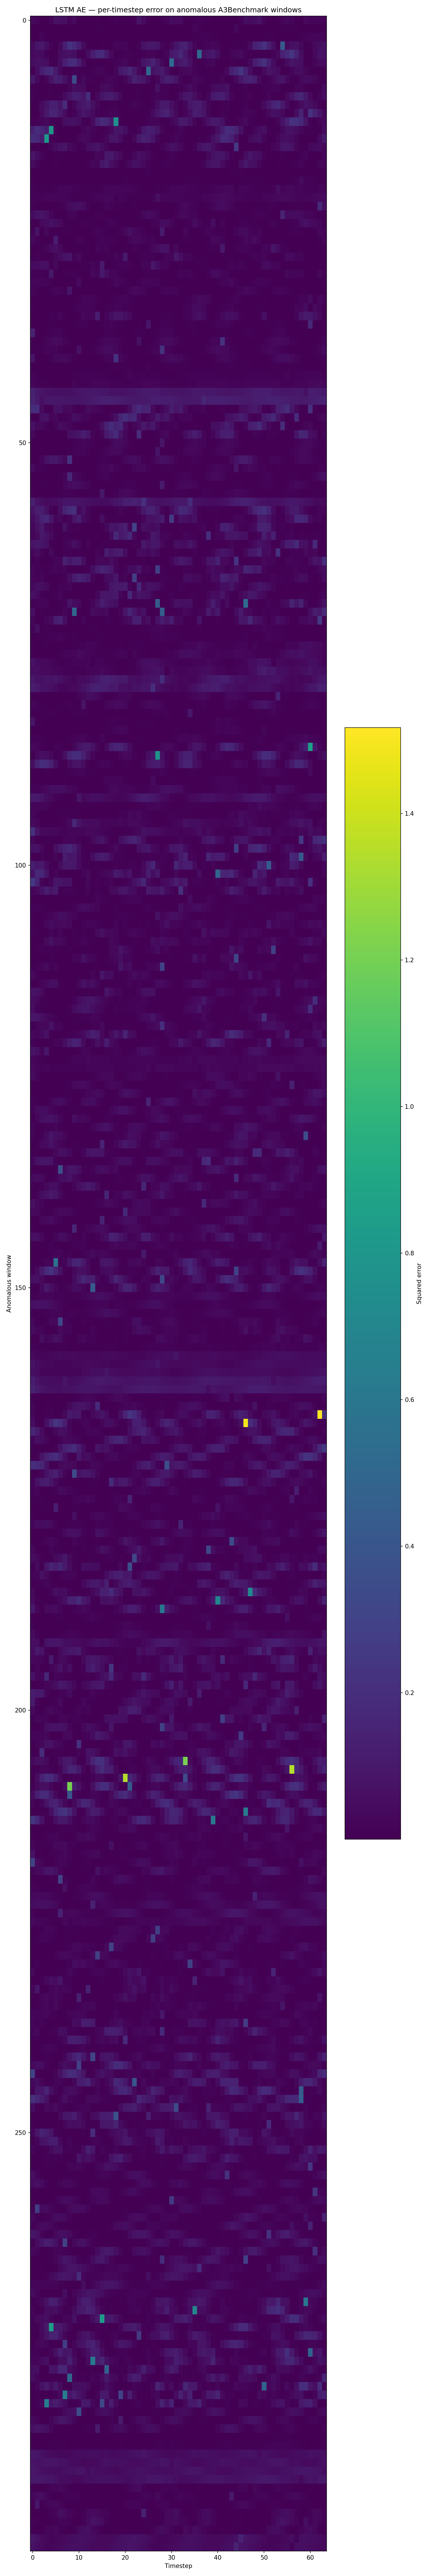
\includegraphics[height=0.4\textheight,keepaspectratio]{../../data/explainability/yahoo_A3Benchmark_lstm_vs_transformer/5/lstm_ae_error_heatmap.png}%
\hspace{0.04\textwidth}%
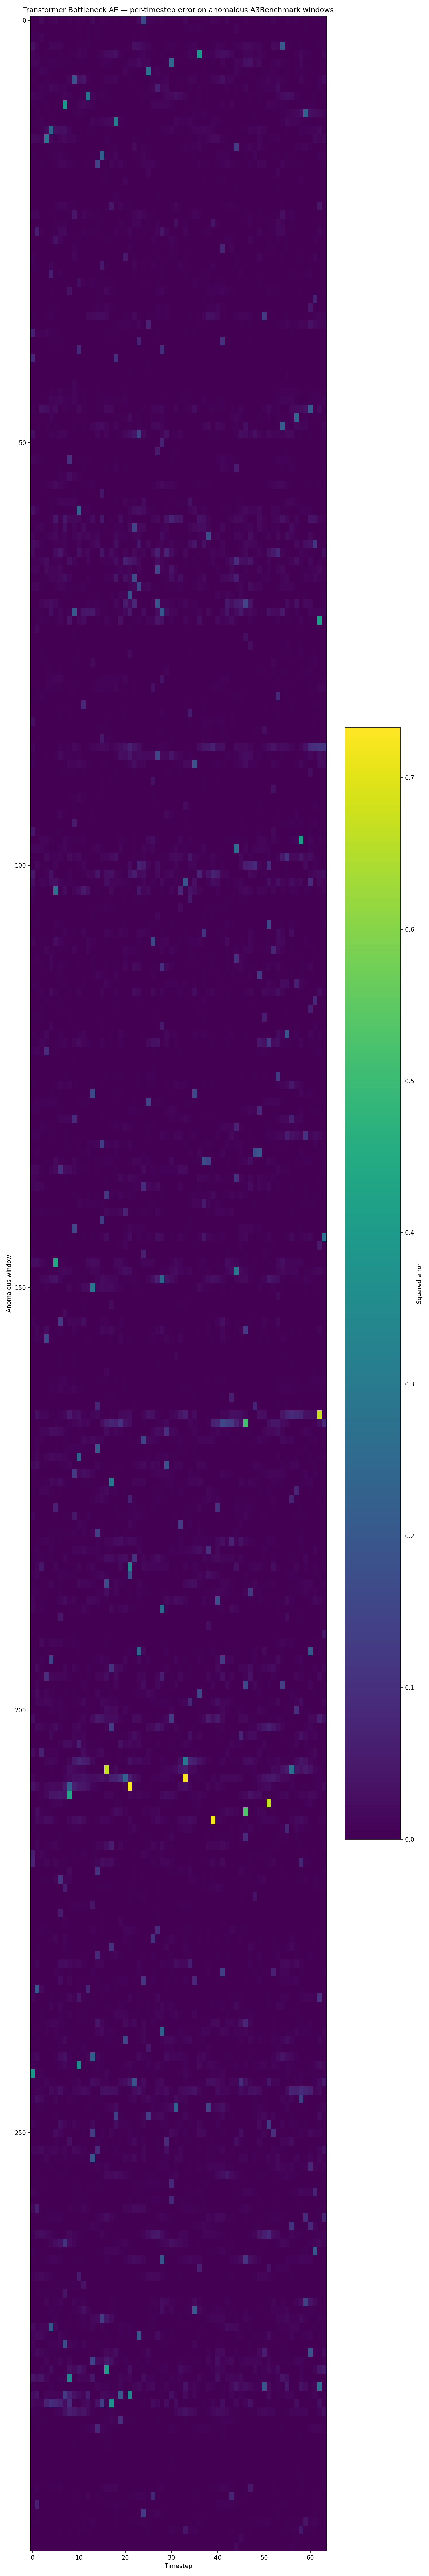
\includegraphics[height=0.4\textheight,keepaspectratio]{../../data/explainability/yahoo_A3Benchmark_lstm_vs_transformer/5/transformer_bottleneck_error_heatmap.png}

\caption{LSTM Autoencoder (stânga) vs.\ Transformer Bottleneck Autoencoder (dreapta) -- eroarea pătratică de reconstrucție per pas temporal pe aceleași 300 de ferestre A3 anormale, eșantionate aleator (câte un rând per fereastră, aceeași ordine a rândurilor). Eroarea ridicată a LSTM AE apare mai des răspândită subțire pe toată lățimea, cu un nivel de bază ușor ridicat pe multe rânduri; eroarea Transformer-ului este vizibil mai rară și limitată la pași temporali izolați.}
\label{fig:explain-lstm-heatmap}
\end{figure}

Comparația vizuală este în linii mari consistentă cu ipoteza inițială -- eroarea Transformer-ului se concentrează în puncte mai puține și mai luminoase, în timp ce eroarea LSTM Autoencoder-ului este mai des răspândită subțire pe toată lățimea unei ferestre. Totuși, harta termică citită cu ochiul liber nu este îndeajuns pentru a confirma mecanismul: fiecare panou este normalizat pe propria sa scală de culoare, iar valorile de eroare ale LSTM Autoencoder-ului sunt, ca magnitudine, aproximativ duble față de cele ale Transformer-ului pe tot parcursul -- de unde necesitatea verificării cantitative din \S\ref{sec:explain-yahoo}.

\chapter{Diagnostice SHAP Suplimentare}
\label{ch:temporal-shap-extra}

Această anexă completează \S\ref{sec:explain-temporal-window} cu doi diagnostici suplimentari pentru atribuirea SHAP a lui Temporal IForest pe ferestre DDoS și DoS slowloris, și \S\ref{sec:explain-disjoint-regime} cu diagrama sumară SHAP a lui AE+Context pe eșantioane PortScan.

\begin{figure}[H]
\centering
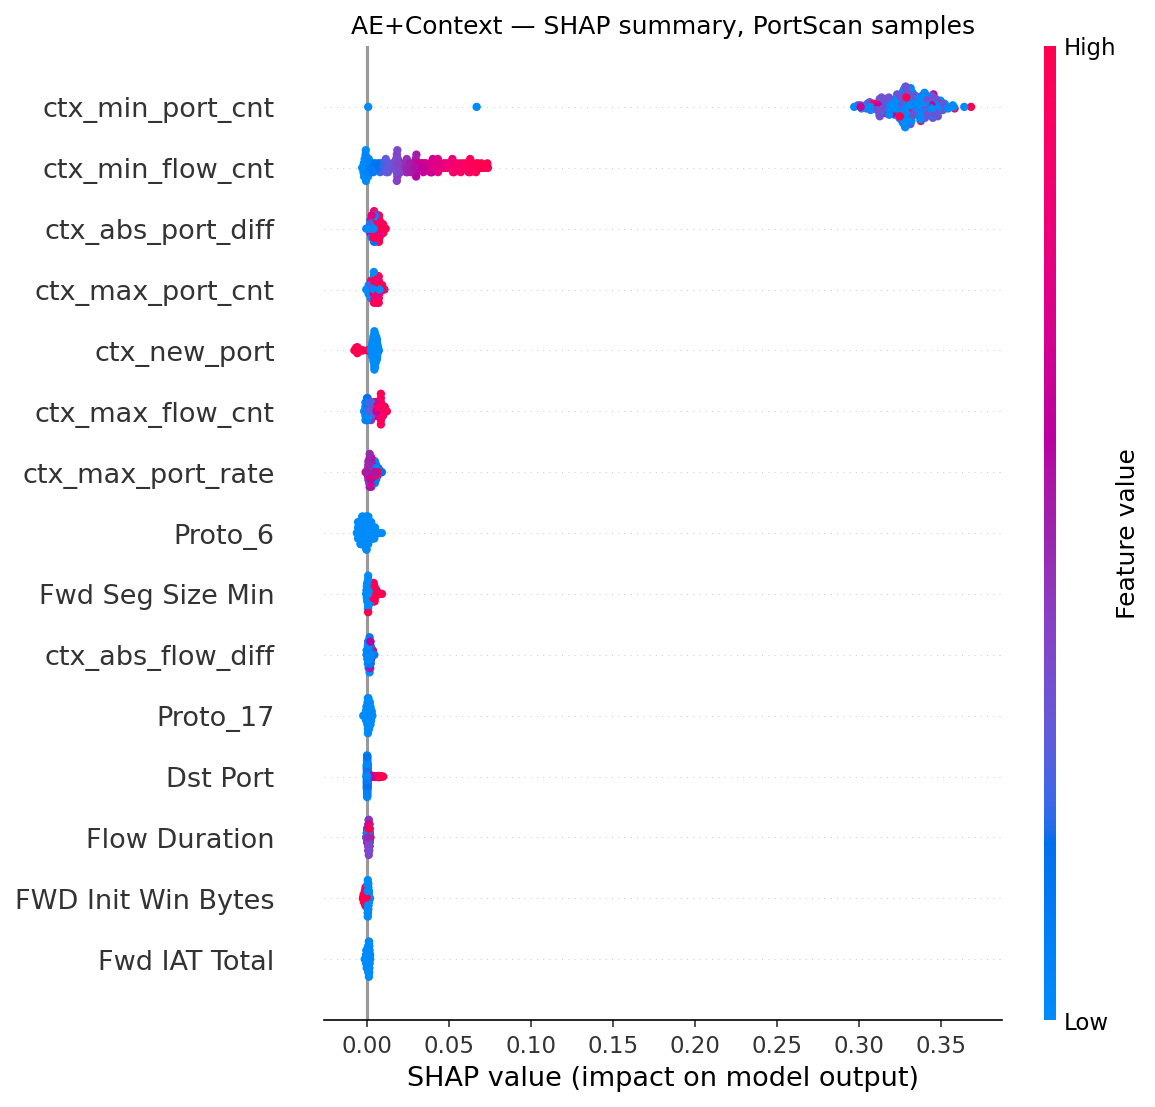
\includegraphics[width=0.65\textwidth]{../../data/explainability/cicids_shap_portscan/5/autoencoder_context_portscan_shap.png}
\caption{AE+Context -- diagramă sumară SHAP, eșantioane PortScan. \texttt{ctx\_min\_port\_cnt} domină printr-un cluster strâns, uniform pozitiv, bine separat de orice altă caracteristică; rândurile de top rămase sunt aproape în întregime caracteristici de context al gazdei.}
\label{fig:explain-ae-context-portscan-shap}
\end{figure}

\begin{figure}[H]
\centering
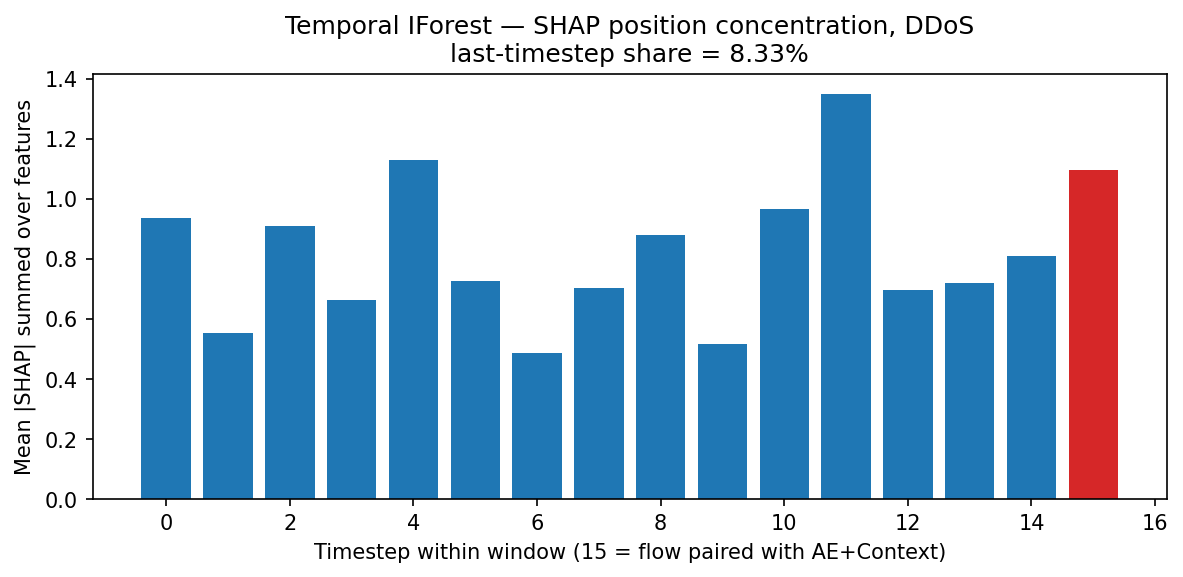
\includegraphics[width=0.48\textwidth,keepaspectratio]{../../data/explainability/cicids_temporal_shap/2/ddos_position_concentration.png}%
\hspace{0.02\textwidth}%
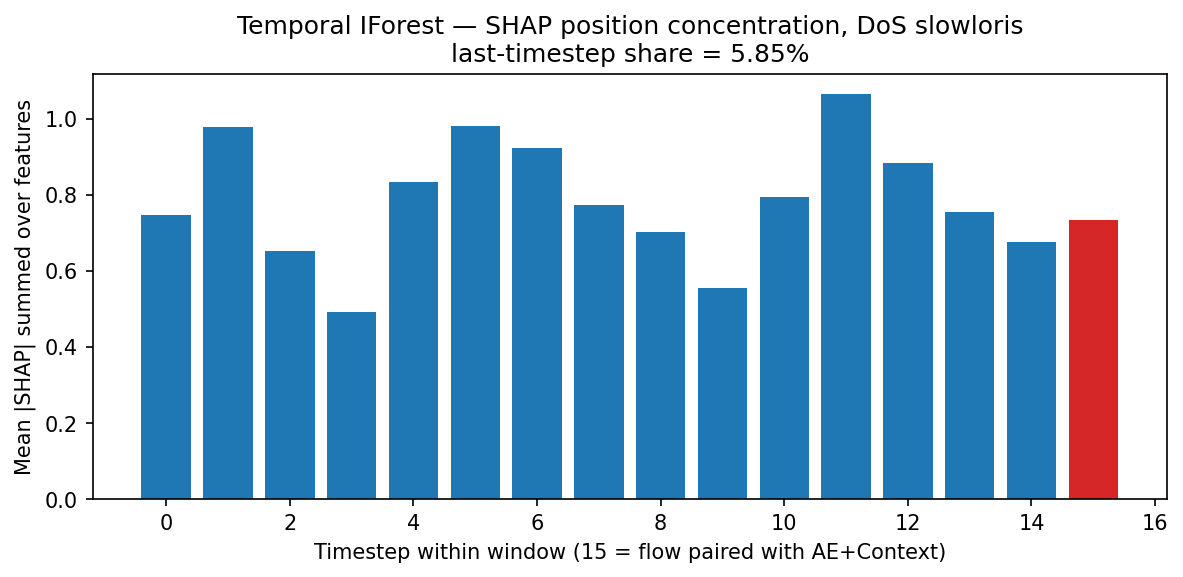
\includegraphics[width=0.48\textwidth,keepaspectratio]{../../data/explainability/cicids_temporal_shap/2/dos_slowloris_position_concentration.png}
\caption{Temporal IForest -- $|\text{SHAP}|$ mediu, sumat pe caracteristici, per pas temporal, ferestre DDoS (stânga) și ferestre DoS slowloris (dreapta). Ultimul pas temporal (bara roșie, 15) -- fluxul combinat cu scorul lui AE+Context în ansamblul propus -- nu poartă mai multă masă de atribuire decât orice altă poziție din fereastră, confirmând statistica sumară raportată în \S\ref{sec:explain-temporal-window}.}
\label{fig:explain-temporal-position-concentration}
\end{figure}

\begin{figure}[H]
\centering
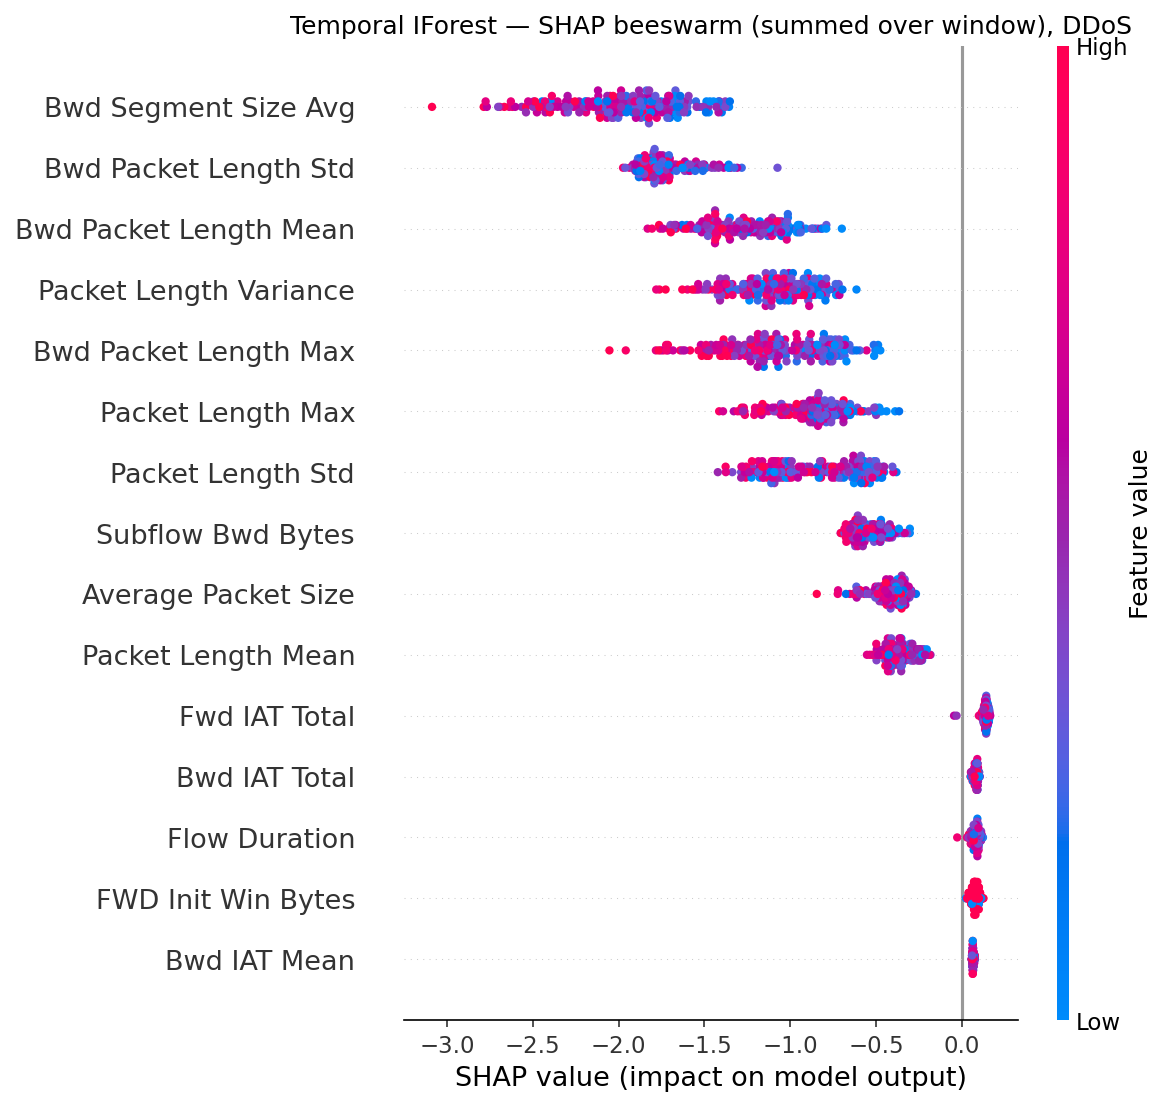
\includegraphics[width=0.48\textwidth,keepaspectratio]{../../data/explainability/cicids_temporal_shap/2/ddos_beeswarm.png}%
\hspace{0.02\textwidth}%
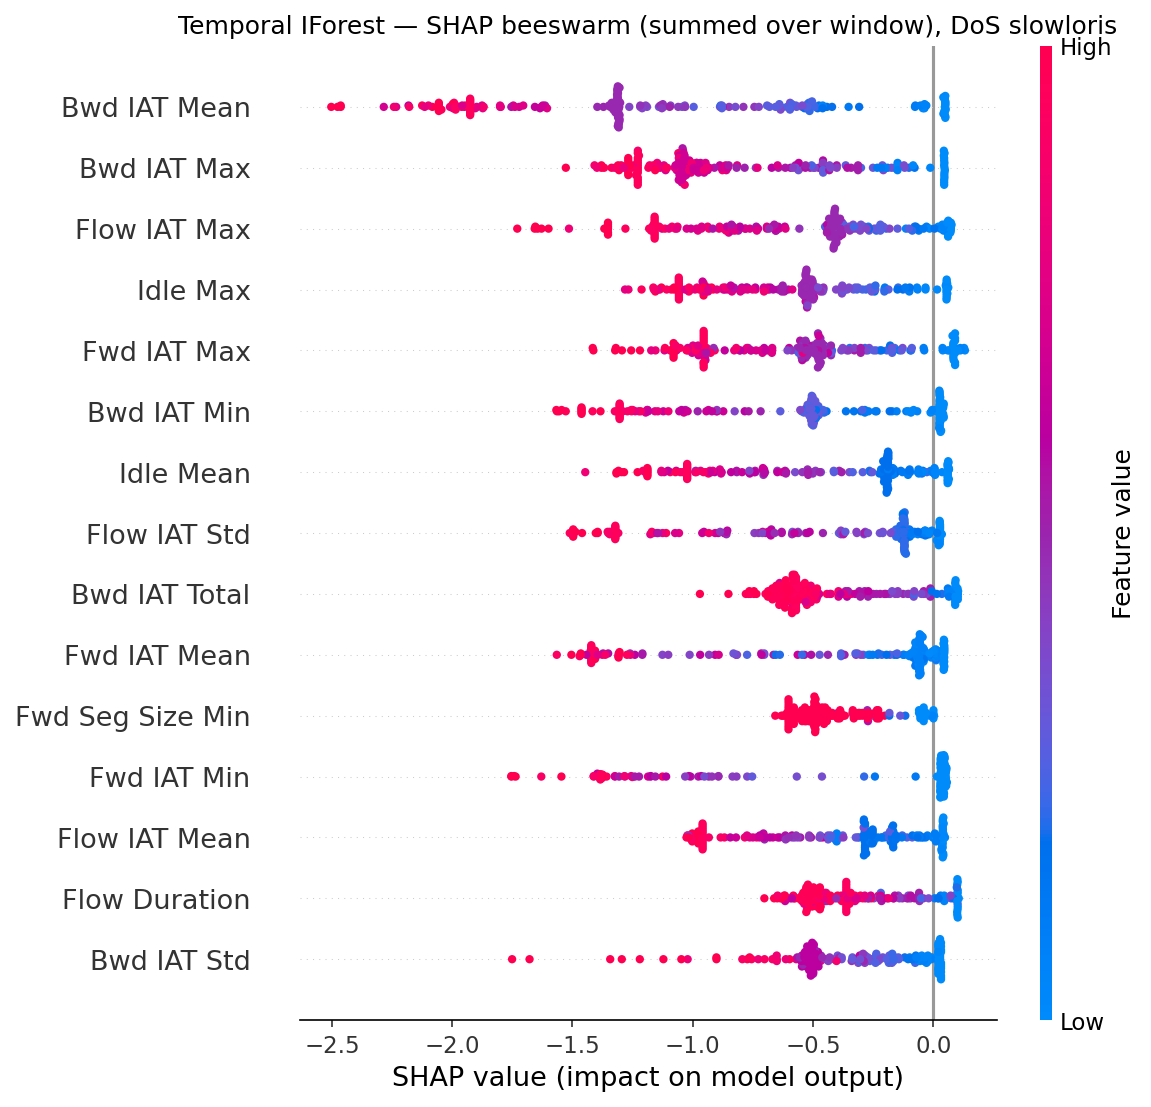
\includegraphics[width=0.48\textwidth,keepaspectratio]{../../data/explainability/cicids_temporal_shap/2/dos_slowloris_beeswarm.png}
\caption{Temporal IForest -- diagramă beeswarm SHAP per caracteristică, ferestre DDoS (stânga) și ferestre DoS slowloris (dreapta), colapsând axa celor 16 pași temporali prin sumarea contribuției SHAP a fiecărei caracteristici pe toată fereastra și colorând după valoarea medie a acelei caracteristici pe fereastră. DoS slowloris arată o relație monotonă clară -- valori mari ale timpului între sosiri (inter-arrival time) determină un SHAP puternic negativ (anormal), valorile mici împing spre zero -- consistent cu comportamentul lent, de menținere a conexiunii, după care este numit atacul. DDoS arată o relație valoare-semn mai zgomotoasă pentru caracteristicile sale de lungime a pachetelor pe direcția inversă, și o răspândire per fereastră mai largă decât sugerează, singură, imaginea de medii din Figura~\ref{fig:explain-temporal-shap}.}
\label{fig:explain-temporal-beeswarm}
\end{figure}

\chapter{Validarea Scorului Temporal IForest Sub Etichetare pe Ultimul Flux}
\label{ch:temporal-iforest-last-flow-validation}

Cifrele de AP per clasă arătate inițial folosesc o etichetă de fereastră "oricare-din-16", adică o fereastră este pozitivă dacă oricare din cele 16 fluxuri ale sale este un atac, etichetată cu tipul de atac majoritar.
Aceasta este mai permisivă decât etichetarea per flux față de care este evaluat AE+Context. Fiecare fereastră de test existentă a fost reetichetată în schimb cu eticheta reală proprie a fluxului \emph{ultim}, iar AP-ul per clasă a fost recalculat față de modelul deja antrenat, neschimbat, și scorurile sale existente.

\begin{center}
\begin{tabular}{@{}lccc@{}}
\toprule
 & AP (oricare-din-16) & AP (ultimul flux) & $n$ (ultimul flux) \\
\midrule
DDoS              & 0.9518 & 0.9515 & 95{,}123 \\
DoS GoldenEye     & 0.6278 & 0.6265 & 7{,}567 \\
DoS Slowhttptest  & 0.6851 & 0.6849 & 1{,}742 \\
DoS slowloris     & 0.6091 & 0.6077 & 4{,}001 \\
Heartbleed        & 0.5927 & 0.2892 & 11 \\
\bottomrule
\end{tabular}
\end{center}

Se observă că AP-ul rămâne practic neschimbat pentru toate cele patru clase țintă sub etichetarea mai strictă, confirmând că scorul este informativ despre statusul propriu al ultimului flux, nu un artefact al etichetării mai permisive.
Heartbleed scade brusc, dar pe doar 11 fluxuri reale -- întreaga sa populație de test -- deci este exclus din ansamblu și tratat ca provizoriu, consistent cu tratamentul său rezervat din Capitolul~\ref{ch:results}.

\chapter{Alinierea Scorurilor și Eșecul Standardizării \texorpdfstring{$z$}{z} pentru Ansamblul AE+Context + Temporal IForest}
\label{ch:ensemble-score-alignment}

Întrucât cele două pipeline-uri de preprocesare reordonează fluxurile diferit înainte de a-și salva propriile array-uri de test (AE+Context sortează global după marca temporală; Temporal IForest sortează per gazdă IP sursă), cele două array-uri de scoruri nu sunt aliniate index-cu-index și trebuie realiniate după identitatea fluxului, recuperând poziția originală a rândului fiecărui flux în intrarea comună, pre-sortare, a ambelor pipeline-uri.


Prima normalizare încercată, standardizarea $z$ (z-scoring) față de media și deviația standard proprii de antrenare benignă ale fiecărui model, s-a dovedit a fi o fundătură, nu un test autentic al niciunei reguli de combinare. Scorurile $z$ de eroare de reconstrucție ale lui AE+Context au cozi extrem de grele (maxim $z \approx 2366$ pe setul de test, cu percentila 99.9 a fluxurilor \emph{benigne} singure deja la $z \approx 227$), în timp ce scorurile $z$ ale lui Temporal IForest rămân strâns mărginite (maxim $z \approx 21$). Sub normalizarea $z$, o mână de valori extreme ale lui AE+Context domină orice combinație liniară sau maxim, indiferent de ponderea alocată lui Temporal IForest: atât regula maximului, cât și fiecare pondere de votare testată au reprodus aproape exact clasamentul propriu al lui AE+Context per clasă (de exemplu, AP-ul GoldenEye a rămas la $0.215$--$0.216$ pe toate cele cinci ponderi, față de $0.215$ al lui AE+Context singur), fără a arăta nicio influență din scorul de sine stătător mult mai puternic al lui Temporal IForest, $0.627$, pe acea clasă. Acesta este un artefact de normalizare, nu o dovadă că metoda combinării nu ajută -- nu testează de fapt ipoteza ansamblului.

Înlocuirea standardizării $z$ cu normalizarea pe rang -- mapând fiecare scor de test la percentila sa în distribuția scorurilor proprii de antrenare benignă ale acelui model, prin funcția de distribuție cumulativă empirică (CDF) -- elimină această problemă prin construcție: fiecare scor normalizat este mărginit la $[0,1]$ indiferent cât de extremă este valoarea brută, deci coada niciunui model nu poate domina coada celuilalt prin simpla magnitudine.

\printbibliography[heading=bibintoc]

\end{document}
